\documentclass[a4paper,11pt,uplatex]{jsarticle}
\usepackage{amsmath,amssymb}
\usepackage{bm}
\usepackage[dvipdfmx]{graphicx}
\usepackage{here}
\usepackage{mypack}
\usepackage{cite}
%テキストの表示領域の調節
\setlength{\textwidth}{\paperwidth}
\addtolength{\textwidth}{-40truemm}
\setlength{\textheight}{\paperheight}
\addtolength{\textheight}{-45truemm}

%余白の調節
\setlength{\topmargin}{-10.4truemm}
\setlength{\evensidemargin}{-5.4truemm}
\setlength{\oddsidemargin}{-5.4truemm}
\setlength{\headheight}{17pt}
\setlength{\headsep}{10mm}
\addtolength{\headsep}{-17pt}
\setlength{\footskip}{5mm}

\title{10.応力解析}
\author{1610004 青木 良太}
\date{提出日 2018年12月6日} % 省略可
\begin{document}
\maketitle

\section{目的}
応力解析とは,物体に荷重が作用した時,物体内に生じている応力(及び歪み)の分布を求めることである.機械設計においては,機械部品・構造における応力集中箇所やその値を求める上で,応力解析が重要な役割を果たしている.
\par
一般に.物体を弾性体と仮定したとしても,応力分布が容易に求められる訳ではない.応力分布が解析的に得られるのは簡単な式で書き下せるような場合のみであり,構造や材料が複雑な場合,応力分布を厳密に求めることは極めて困難
となる.そのような状況においても解を得る手段として応力分布を求める基礎方程式を近似式に置き換え,具体的な荷重や変位拘束条件を与えて近似解を数値的に計算する数値解放と呼ばれる方法が用いられる.
\par
この実験では,応力解析を行う上で代表的な数値解法である有限要素法の入門的な訓練を行う.構造解析に源をもつこの有限要素法は,今日では工学のあらゆる分野で利用されている.
第1週目では,有限要素法の基礎の習得を目的としてトラスの応力解析を実施し,第2週目には円孔のある平板の2次元有限要素法を実施する.

\section{理論}
\subsection{トラスの有限要素解析}
\subsubsection{トラス構造}
トラス構造とは,棒状の複数の部材がピン結合によってつなぎ合わ亜された構造であり,ここの部材には軸力のみが伝達され,はりのような横荷重/曲げモーメントは受けない.部材の断面形状,並びに弾性係数(ヤング率)
が一様であれば,それぞれの部材内の応力も一様となる.
\par
トラスの構造解析においては,まず各要素毎に要素剛性方程式と呼ばれる方程式を立て,次に要素方程式から全体剛性方程式を組み立ててトラス全体の解析を行う.
\subsection{要素剛性方程式の導出}
ここでは,各要素ごとに成立する力学関係について調べ,方程式を導出する.以降において,ことわりのない限り右向きを正とする.
図\ref{棒材}のような長さ$L$,断面積$A$,ヤング率$E$の一様な棒材の両端に$f_1,f_2$の力が加わって$u_1,u_2$の変位が生じているとする.

\begin{figure}[H]
  \begin{center}
    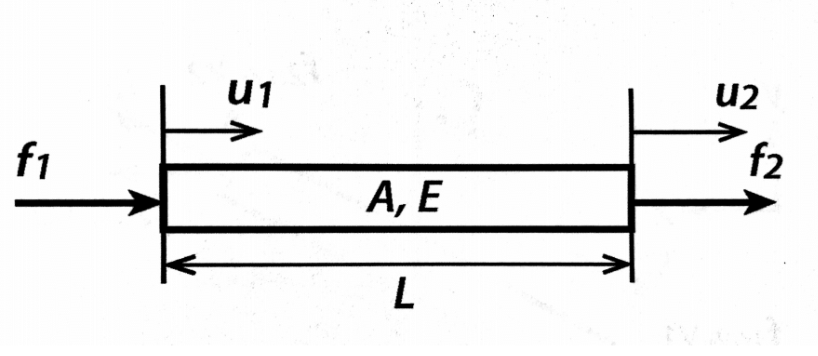
\includegraphics[width = 8cm]{画像/stick.png}
    \caption{一様な棒材}
    \label{棒材}
  \end{center}
\end{figure}

このときひずみは
\begin{align}
  \epsilon = \frac{u_2-u_1}{L}
\end{align}
であり, 棒材内に作用する応力は
\begin{align}
  \sigma = E\epsilon = \frac{E}{L}(u_2-u_1)
\end{align}
となる.ただし,応力は引っ張り方向を正,圧縮方向を負とする.すなわち,
\begin{align}
  \label{3}
  f_1 &= -\sigma A = -\frac{AE}{L}(u_2 - u_1) \\
  f_2 &= \sigma \frac{AE}{L}(u_2 - u_1)
\end{align}
となる.式(\ref{3})より,明らかに$f_1 + f_2 = 0$であり,力のつりあい関係が満たされている.式(\ref{3})は,行列を用いて次のようにまとめられる.
\begin{align}
  \label{4}
  \pmat{f_1 \\ f_2} = \frac{AE}{L} \pmat{1 & -1 \\ -1 & 1} \pmat{u_1 \\ u_2}
\end{align}
式(\ref{4})は,要素剛性方程式と呼ばれるトラス構造解析における基礎式である.また,式(\ref{4})の右辺の係数行列を要素剛性行列と呼ぶ.
\par
次に,図\ref{xy棒材}のような二次元平面状に偏角$\theta$で傾いた長さ$l_a$の棒要素$a$について考える.要素$a$の断面積とヤング率はそれぞれ$A_a, E_a$である.

\begin{figure}[H]
  \begin{center}
    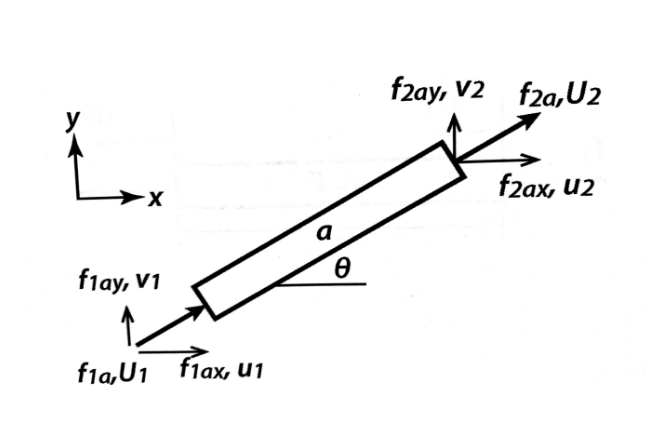
\includegraphics[width = 8cm]{画像/xystick.png}
    \caption{偏角$\theta$での$xy$平面状に置かれた棒材}
    \label{xy棒材}
  \end{center}
\end{figure}

両端1,2から,要素$a$に加える力$f_{1ax},f_{1ay},f_{2ax},f_{2ay}$と変位$u_1,v_1,u_2,v_2$との間に成り立つ関係式は,両端に加える力を$f_{1a},f_{2a}$,変位を$U_1,U_2$とすれば,式\ref{4}
より,要素剛性方程式
\begin{align}
  \pmat{f_{1a} \\ f_{2a}} = k_a \pmat{1 & -1 \\ -1 & 1} \pmat{U_1 \\ U_2}
\end{align}
が成り立つ.ここで$k_a = A_a  E_a / L_a$は要素$a$のバネ定数である.節点力及び変位を$x,y$成分で表示すれば,
\begin{align}
  \pmat{f_{1ax} \\ f_{1ay} \\ f_{2ax} \\ f_{2ay}} = \pmat{f_{1a} \cos \theta \\ f_{1a} \sin \theta \\ f_{2a} \cos \theta \\ f_{2a} \sin \theta} =
  \pmat{\cos \theta & 0 \\ \sin \theta & 0 \\ 0 & \cos \theta \\ 0 & \sin \theta} \pmat{f_{1a} \\ f_{2a}}
\end{align}
及び,
\begin{align}
  \pmat{U_1 \\ U_2} = \pmat{\cos \theta & \sin \theta & 0 & 0 \\ 0 & 0 & \cos \theta & \sin \theta} \pmat{u_1 \\ v_1 \\ u_2 \\ v_2}
\end{align}
とかけるから,
\begin{align}
  \pmat{f_{1ax} \\ f_{1ay} \\ f_{2ax} \\ f_{2ay}} &= k_a \pmat{\cos \theta & 0 \\ \sin \theta & 0 \\ 0 & \cos \theta \\ 0 & \sin \theta} \pmat{1 & -1 \\ -1 & 1}
  \pmat{\cos \theta & \sin \theta & 0 & 0 \\ 0 & 0 & \cos \theta & \sin \theta} \pmat{u_1 \\ v_1 \\ u_2 \\ v_2} \\
  \label{8}
  &= k_a \pmat{\cos^2 \theta & \cos \theta \sin \theta & -\cos^2 \theta & -\cos \theta \sin \theta \\ \cos \theta \sin \theta & \sin^2 \theta & -\cos \theta \sin \theta
  & -\sin^2 \theta \\ -\cos^2 \theta & -\cos \theta \sin \theta & \cos^2 \theta & \cos \theta \sin \theta \\ -\cos \theta \sin \theta & -\sin^2 \theta& \cos \theta \sin \theta
  & \sin^2 \theta} \pmat{u_1 \\ v_1 \\ u_2 \\ v_2}
\end{align}
となる. これが,偏角$\theta$で傾いた要素$a$に関する要素剛性方程式である.

\subsubsection{全体剛性方程式の導出}
前節で導出した要素剛性方程式を組み合わせて,一つの方程式にまとめることで,トラス構造全体の剛性方程式を導くことができる.

\begin{figure}[H]
  \begin{center}
    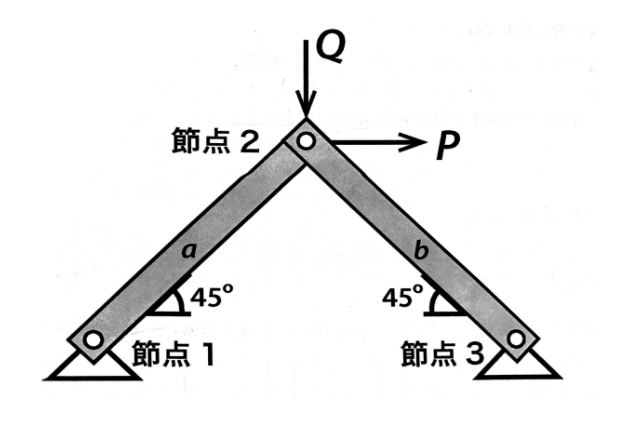
\includegraphics[width = 8cm]{画像/trus.png}
    \caption{二要素のトラス}
    \label{2トラス}
  \end{center}
\end{figure}

図\ref{2トラス}のような2要素トラス構造に以下のように接点力,変位を考える.\\
$f_{ijk}$:節点$i$が要素$j$に及ぼす$k$方向の力 \\
$u_i$:節点$i$の$x$方向の変位 \\
$v_i$:接点$i$の$y$方向の変位 \\

要素剛性方程式(\ref{8})をそれぞれの要素に適用すると,それぞれ以下のように表される.

\begin{align}
  \label{9}
  \pmat{f_{1ax} \\ f_{1ay} \\ f_{2ax} \\ f_{2ay}} &=  k_a \pmat{\cos^2 \theta_a & \cos \theta_a \sin \theta_a & -\cos^2 \theta_a & -\cos \theta_a \sin \theta_a \\ \cos \theta_a \sin \theta_a & \sin^2 \theta_a & -\cos \theta_a \sin \theta_a
  & -\sin^2 \theta_a \\ -\cos^2 \theta_a & -\cos \theta_a \sin \theta_a & \cos^2 \theta_a & \cos \theta_a \sin \theta_a \\ -\cos \theta_a \sin \theta_a & -\sin^2 \theta_a& \cos \theta_a \sin \theta_a
  & \sin^2 \theta_a} \pmat{u_1 \\ v_1 \\ u_2 \\ v_2} \\
  \label{10}
  \pmat{f_{1bx} \\ f_{1by} \\ f_{2bx} \\ f_{2by}} &= k_b \pmat{\cos^2 \theta_b & \cos \theta_b \sin \theta_b & -\cos^2 \theta_b & -\cos \theta_b \sin \theta_b \\ \cos \theta_b \sin \theta_b & \sin^2 \theta_b & -\cos \theta_b \sin \theta_b
  & -\sin^2 \theta_b \\ -\cos^2 \theta_b & -\cos \theta_b \sin \theta_b & \cos^2 \theta_b & \cos \theta_b \sin \theta_b \\ -\cos \theta_b \sin \theta_b & -\sin^2 \theta_b & \cos \theta_b \sin \theta_b
  & \sin^2 \theta_b} \pmat{u_1 \\ v_1 \\ u_2 \\ v_2}
\end{align}

ここで,各節点における力のつりあいを考えると以下のようになる.
\begin{description}
  \item[節点1] 
  \begin{align}
    f_{1x} &= f_{1ax} \\
    f_{1y} &= f_{1ay}
  \end{align}
  \item[節点2] 
  \begin{align}
    f_{2x} &= f_{2ax} + f_{2bx} \\
    f_{2y} &= f_{2ay} + f_{2by}
  \end{align}
  \item[節点3]
  \begin{align}
    f_{3x} &= f_{3bx} \\
    f_{3y} &= f_{3by}
  \end{align}
\end{description}

この関係をベクトルを用いて整理すると,
\begin{align}
  \pmat{f_{1x} \\ f_{1y} \\ f_{2x} \\ f_{2y} \\ f_{3x} \\f_{3y}} = \pmat{f_{1ax} \\ f_{1ay} \\ f_{2ax} \\ f_{2ay} \\ 0\\0} +
  \pmat{0 \\ 0 \\f_{2bx} \\ f_{2by} \\ f_{3bx} \\ f_{3by}} = \pmat{f_{1ax} \\ f_{1ay} \\ f_{2ax} + f_{2bx} \\ f_{2ay} + f_{2by} \\ f_{3bx} \\ f_{3by}}
\end{align}
のように表される.なお,各要素に作用する節点力ベクトルが4成分であるのに対し,考える構造体に作用する節点力ベクトルは6成分となることから,
要素の節点力ベクトルに対して適宜6成分ベクトルになるように修正した.さらに,式(\ref{9}),(\ref{10})の変位を6成分とした場合でも要素剛性方程式が成り立つように要素剛性行列に0を補うと,
\begin{align}
  \label{12}
  \pmat{f_{1ax} \\ f_{1ay} \\ f_{2ax} \\ f_{2ay} \\ f_{3ax} \\ f_{3ay}} &= k_a \pmat{\cos^2 \theta_a & \cos \theta_a \sin \theta_a & -\cos^2 \theta_a & -\cos \theta_a \sin \theta_a &0&0 \\ \cos \theta_a \sin \theta_a & \sin^2 \theta_a & -\cos \theta_a \sin \theta_a
  & -\sin^2 \theta_a &0 &0\\ -\cos^2 \theta_a & -\cos \theta_a \sin \theta_a & \cos^2 \theta_a & \cos \theta_a \sin \theta_a &0&0\\ -\cos \theta_a \sin \theta_a & -\sin^2 \theta_a& \cos \theta_a \sin \theta_a
  & \sin^2 \theta_a &0&0 \\ 0&0&0&0&0&0 \\ 0&0&0&0&0&0} \pmat{u_1 \\ v_1 \\ u_2 \\ v_2 \\ u_3 \\ v_3} \\
  \label{13}
  \pmat{f_{1bx} \\ f_{1by} \\ f_{2bx} \\ f_{2by}} &= k_b \pmat{0&0&0&0&0&0 \\ 0&0&0&0&0&0 \\ 0&0& \cos^2 \theta_b & \cos \theta_b \sin \theta_b & -\cos^2 \theta_b & -\cos \theta_b \sin \theta_b \\ 0&0&\cos \theta_b \sin \theta_b & \sin^2 \theta_b & -\cos \theta_b \sin \theta_b
  & -\sin^2 \theta_b \\ 0&0&-\cos^2 \theta_b & -\cos \theta_b \sin \theta_b & \cos^2 \theta_b & \cos \theta_b \sin \theta_b \\ 0&0&-\cos \theta_b \sin \theta_b & -\sin^2 \theta_b & \cos \theta_b \sin \theta_b
  & \sin^2 \theta_b} \pmat{u_1 \\ v_1 \\ u_2 \\ v_2 \\ u_3 \\ v_3}
\end{align}
となる.式(\ref{12}),(\ref{13})をそれぞれ足し合わせることで,構造全体の剛性方程式が
\begin{align}
  \pmat{f_{1x} \\ f_{1y} \\ f_{2x} \\ f_{2y} \\ f_{3x} \\f_{3y}} = \pmat{k_a C_aC_a & k_aC_aS_a& -k_aC_a C_a &-k_a C_aS_a&0&0 \\ k_aC_aS_a& k_aS_aS_a& -k_aC_aS_a
  & -k_aS_aS_a&0 &0\\ -k_aC_aC_a& -k_aC_aS_a & k_aC_aC_a + k_b C_bC_b& k_aC_aS_a +k_bC_bS_b &-k_bC_bC_b&-k_bC_bS_b\\ -k_aC_aS_a& -k_aS_aS_a& k_aC_aS_a + k_bC_bS_b
  & k_aS_aS_a + k_bS_bS_b&-k_bC_bS_b&-k_bS_bS_b \\ 0&0&-k_bC_bC_b & -k_bC_bS_b& k_bC_bC_b& k_bC_bS_b \\ 0&0&-k_bC_bS_b&-k_bS_bS_b &-k_bC_bS_b & k_bS_bS_b}
\end{align}
のように得られる.

\subsection{平面応力解析}
薄板などの平面構造に関する応力解析を考える.トラス構造は線形変形する要素によって構成されているが,平面構造にはそのような要素がない.そのため,応力解析の実施にあたってはまず,解析しようとする平面領域を
三角形や四角形の小領域に仮想敵に分割する必要がある.この時用いられる三角形や四角形を要素と呼び,それぞれの頂点を節点と呼ぶ.
\par
三角形要素$a$を考え,節点$i$が要素$a$に加える力を($f_{iax},f_{iay}$),変位を($u_i,v_i$)とする(ただし$i = 1,2,3$).
今,弾性体の微笑変形を考え,三角形要素内の任意の変位($u,v$)が線形関係となることを仮定すると,
\begin{align}
  u = \alpha_0 + \alpha_1 x + \alpha_2 y \\
  v = \beta_0 +\beta_1 x + \beta_2 y
\end{align}
のように表される.この時,これらの係数と変位との関係式が各節点座標$x_1,y_1$を用いて
\begin{align}
  \label{17}
  \pmat{u_1 \\ v_1 \\ u_2 \\ v_2 \\ u_3 \\ v_3} = \pmat{1 & 0 & x_1 & 0 & y_1 & 0 \\ 0 & 1 & 0 & x_1 & 0 & y_1 \\
  1 & 0 & x_2 & 0 & y_2 & 0 \\ 0 & 1 & 0 & x_2 & 0 & y_2 \\ 1 & 0 & x_3 & 0 & y_3 & 0 \\ 0 & 1 & 0 & x_3 & 0 & y_3}
  \pmat{\alpha_0 \\ \beta_0 \\ \alpha_1 \\ \beta_1 \\ \alpha_2 \\ \beta_2}
\end{align}
のように表される.材料力学あるいは弾性論より,変位と歪みの関係式は
\begin{align}
  \epsilon_x &= \frac{\partial{u}}{\partial{x}} = \alpha_1 \\
  \epsilon_y &= \frac{\partial{v}}{\partial{y}} = \beta_2 \\
  \gamma_{xy} &= \frac{\partial{v}}{\partial{x}} + \frac{\partial{u}}{\partial{y}} = \alpha_2 + \beta_1
\end{align}

で与えられる.これと式\ref{17}を用いれば,歪みと節点座標との関係式が導出できる.さらに,応力-歪み関係式を用いることで,節点力と変位との関係式,すなわち三角形要素の要素剛性方程式
\begin{align}
  \pmat{f_{1ax} \\ f_{1ay} \\ f_{2ax} \\ f_{2ay} \\ f_{3ax} \\ f_{3ay}} = A \pmat{u_1 \\ v_1 \\ u_2 \\ v_2 \\ u_3 \\ v_3}
\end{align}

が導出される.ここで,$A$は$6 \times 6$の要素剛性行列で,三角形要素の節点座標と弾性定数から定まる.
\par
その後のプロセスはトラス解析と全く同じである.すなわち,要素剛性方程式を組み合わせ,全体剛性方程式を作る.これは,全ての節点に加わる外力と節点の線形方程式である.各節点で,$x,y$方向に関して,
変位または力のいずれかは拘束条件として与え,未知の節点変位を連立1次方程式から決定する.変位が決まれば,要素の歪み及び応力が求められる.
\par
重要な点は,ここで導入した三角形要素の要素内での応力・歪みが一定値となることである.すなわち,応力や歪みの急変部では,十分に細かい要素を用いなければ近似が粗くなる.

\section{実験方法}
\subsection{トラスの有限要素解析}
図\ref{2トラス},\ref{trus_a},\ref{trus_b},\ref{truss11}に示すトラス構造について有限要素解析を行った.
各トラス構造において節点と要素に番号をつけ,節点の座標とともにテキストファイルに記した.
この時,P=15kN,Q=10kN L=2.0m, A=100$\mathrm{mm^2}$,E=200GPa(2トラスの場合),P=30kN, L=3.0m, A=200$\mathrm{mm^2}$,E=70GPa(その他の場合)とした.
作成したテキストファイルをトラス構造解析プログラムに読み込ませ,構造解析を行った.

\begin{figure}[H]
  \begin{center}
    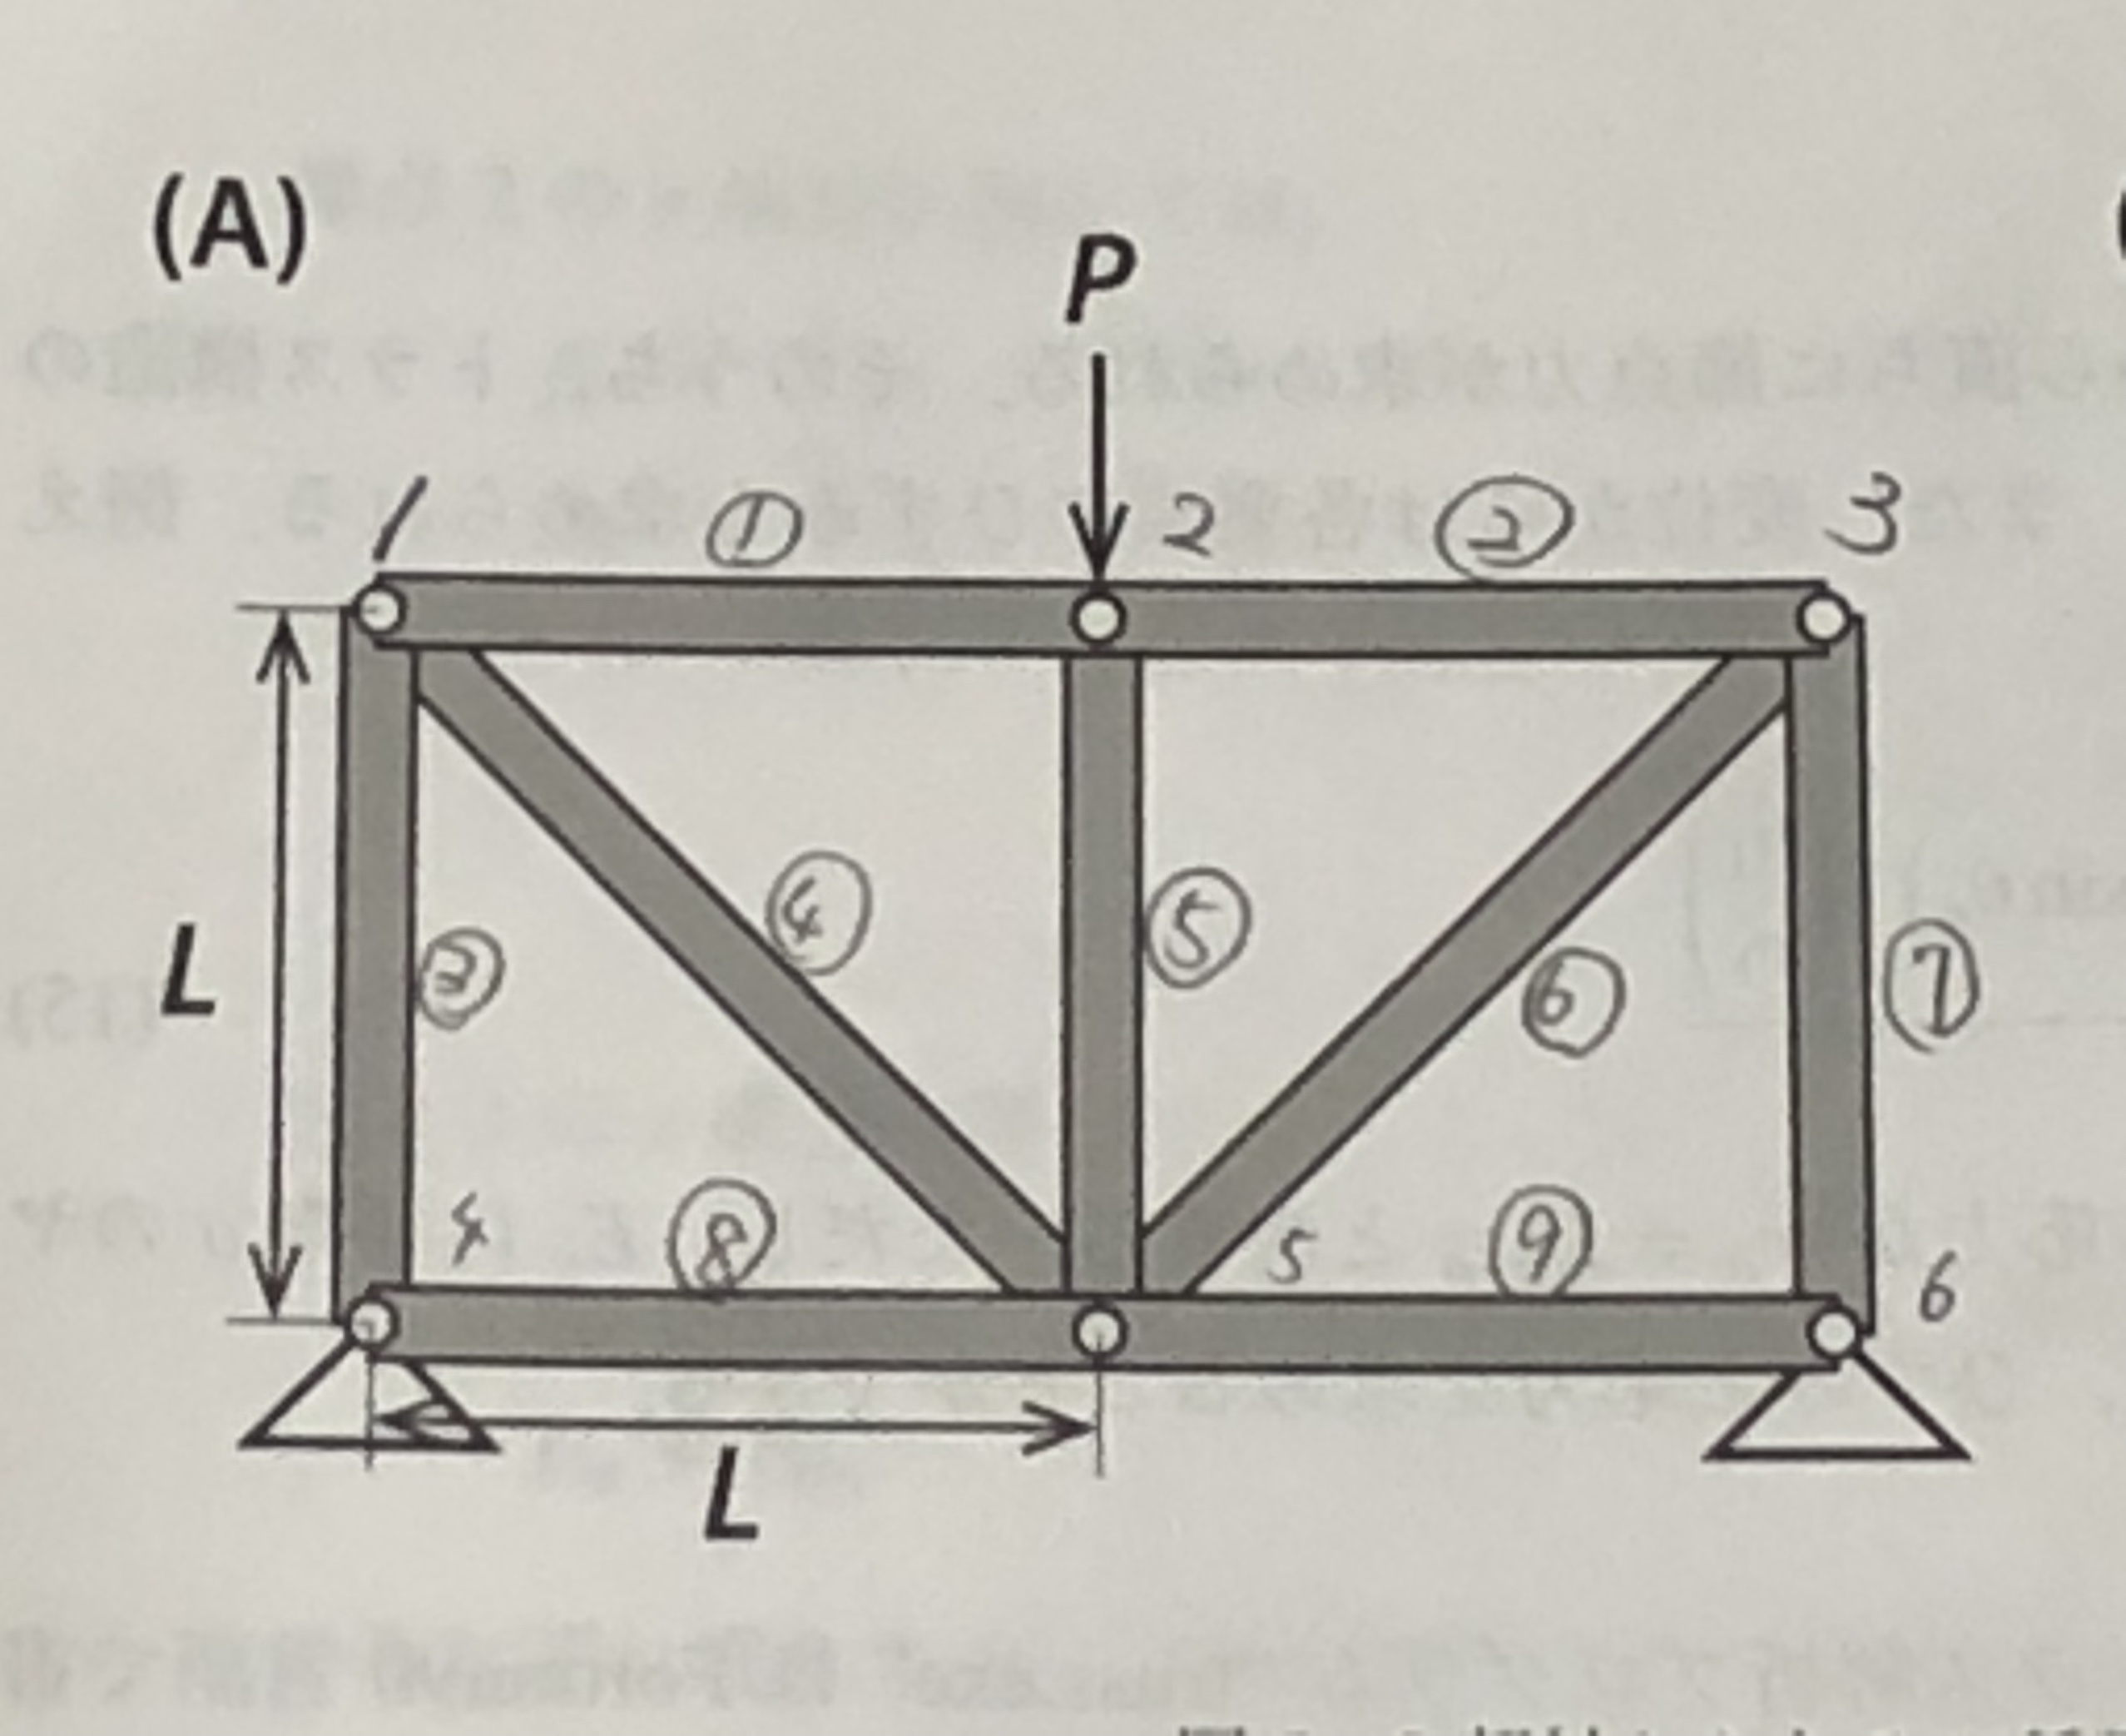
\includegraphics[width = 8cm]{画像/trus_a.JPG}
    \caption{9部材からなる2種類のトラス構造(A)}
    \label{trus_a}
  \end{center}
\end{figure}

\begin{figure}[H]
  \begin{center}
    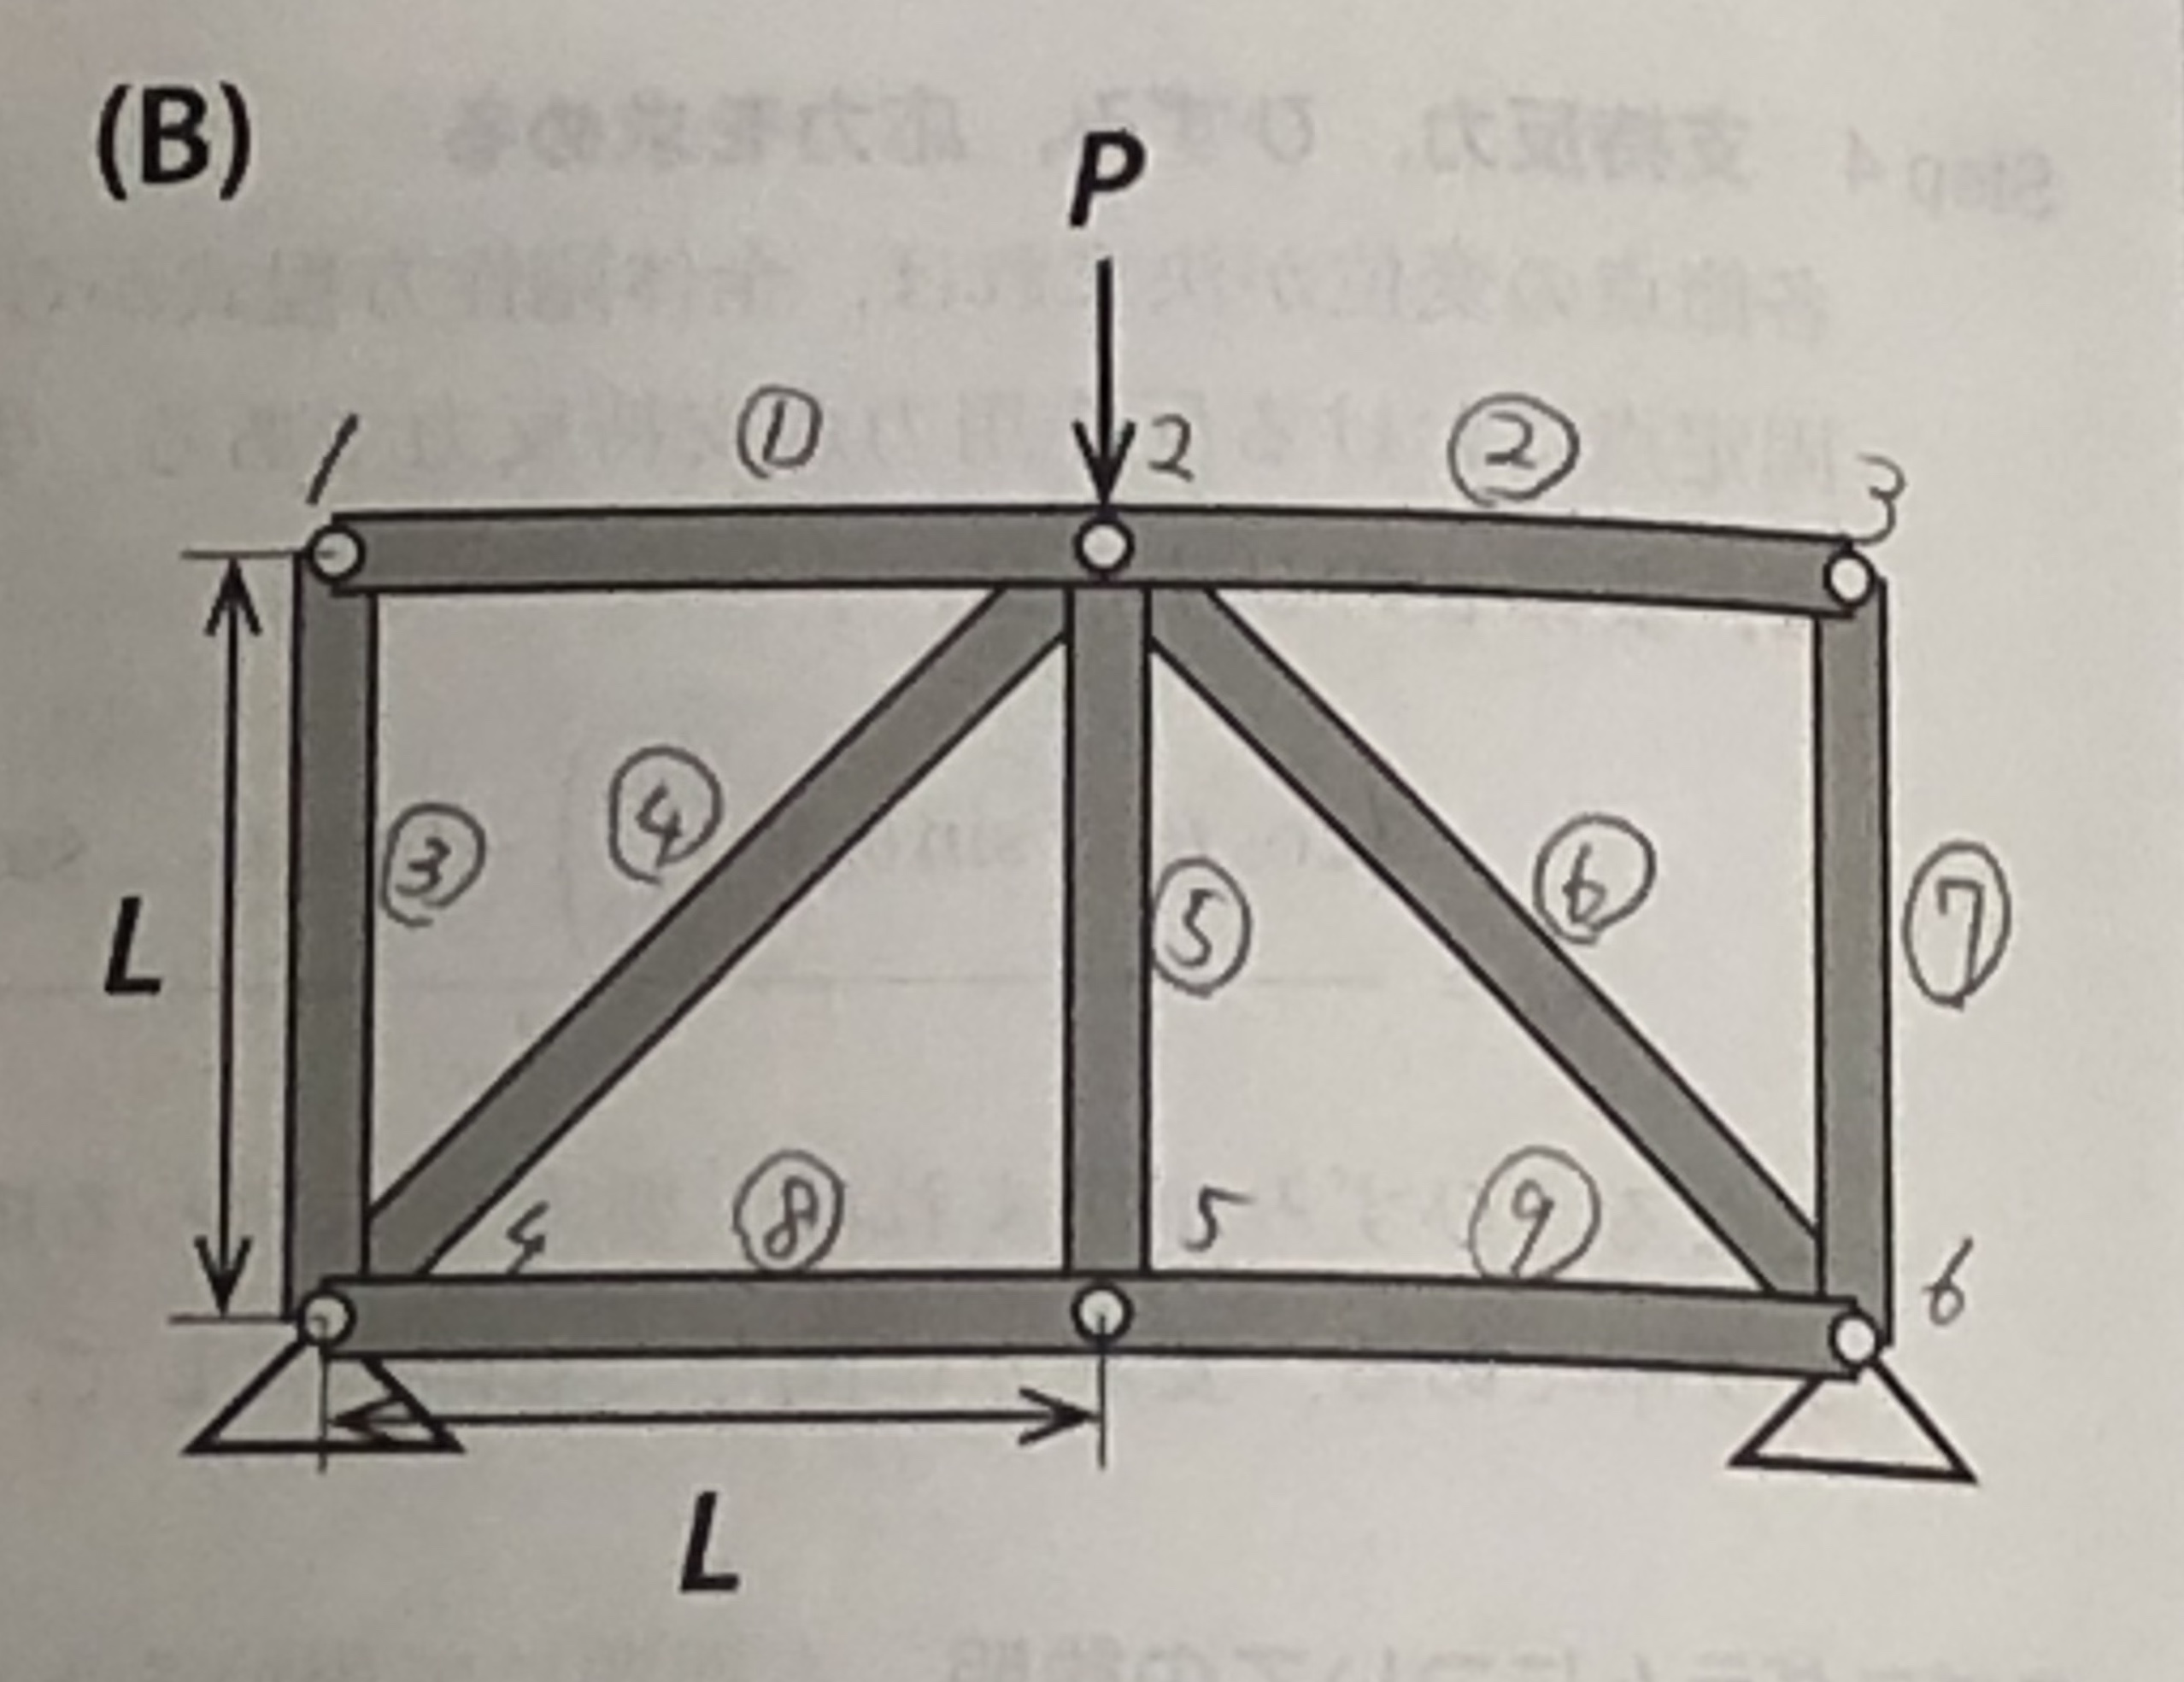
\includegraphics[width = 8cm]{画像/trus_b.JPG}
    \caption{9部材からなる2種類のトラス構造(B)}
    \label{trus_b}
  \end{center}

\end{figure}
\begin{figure}[H]
  \begin{center}
    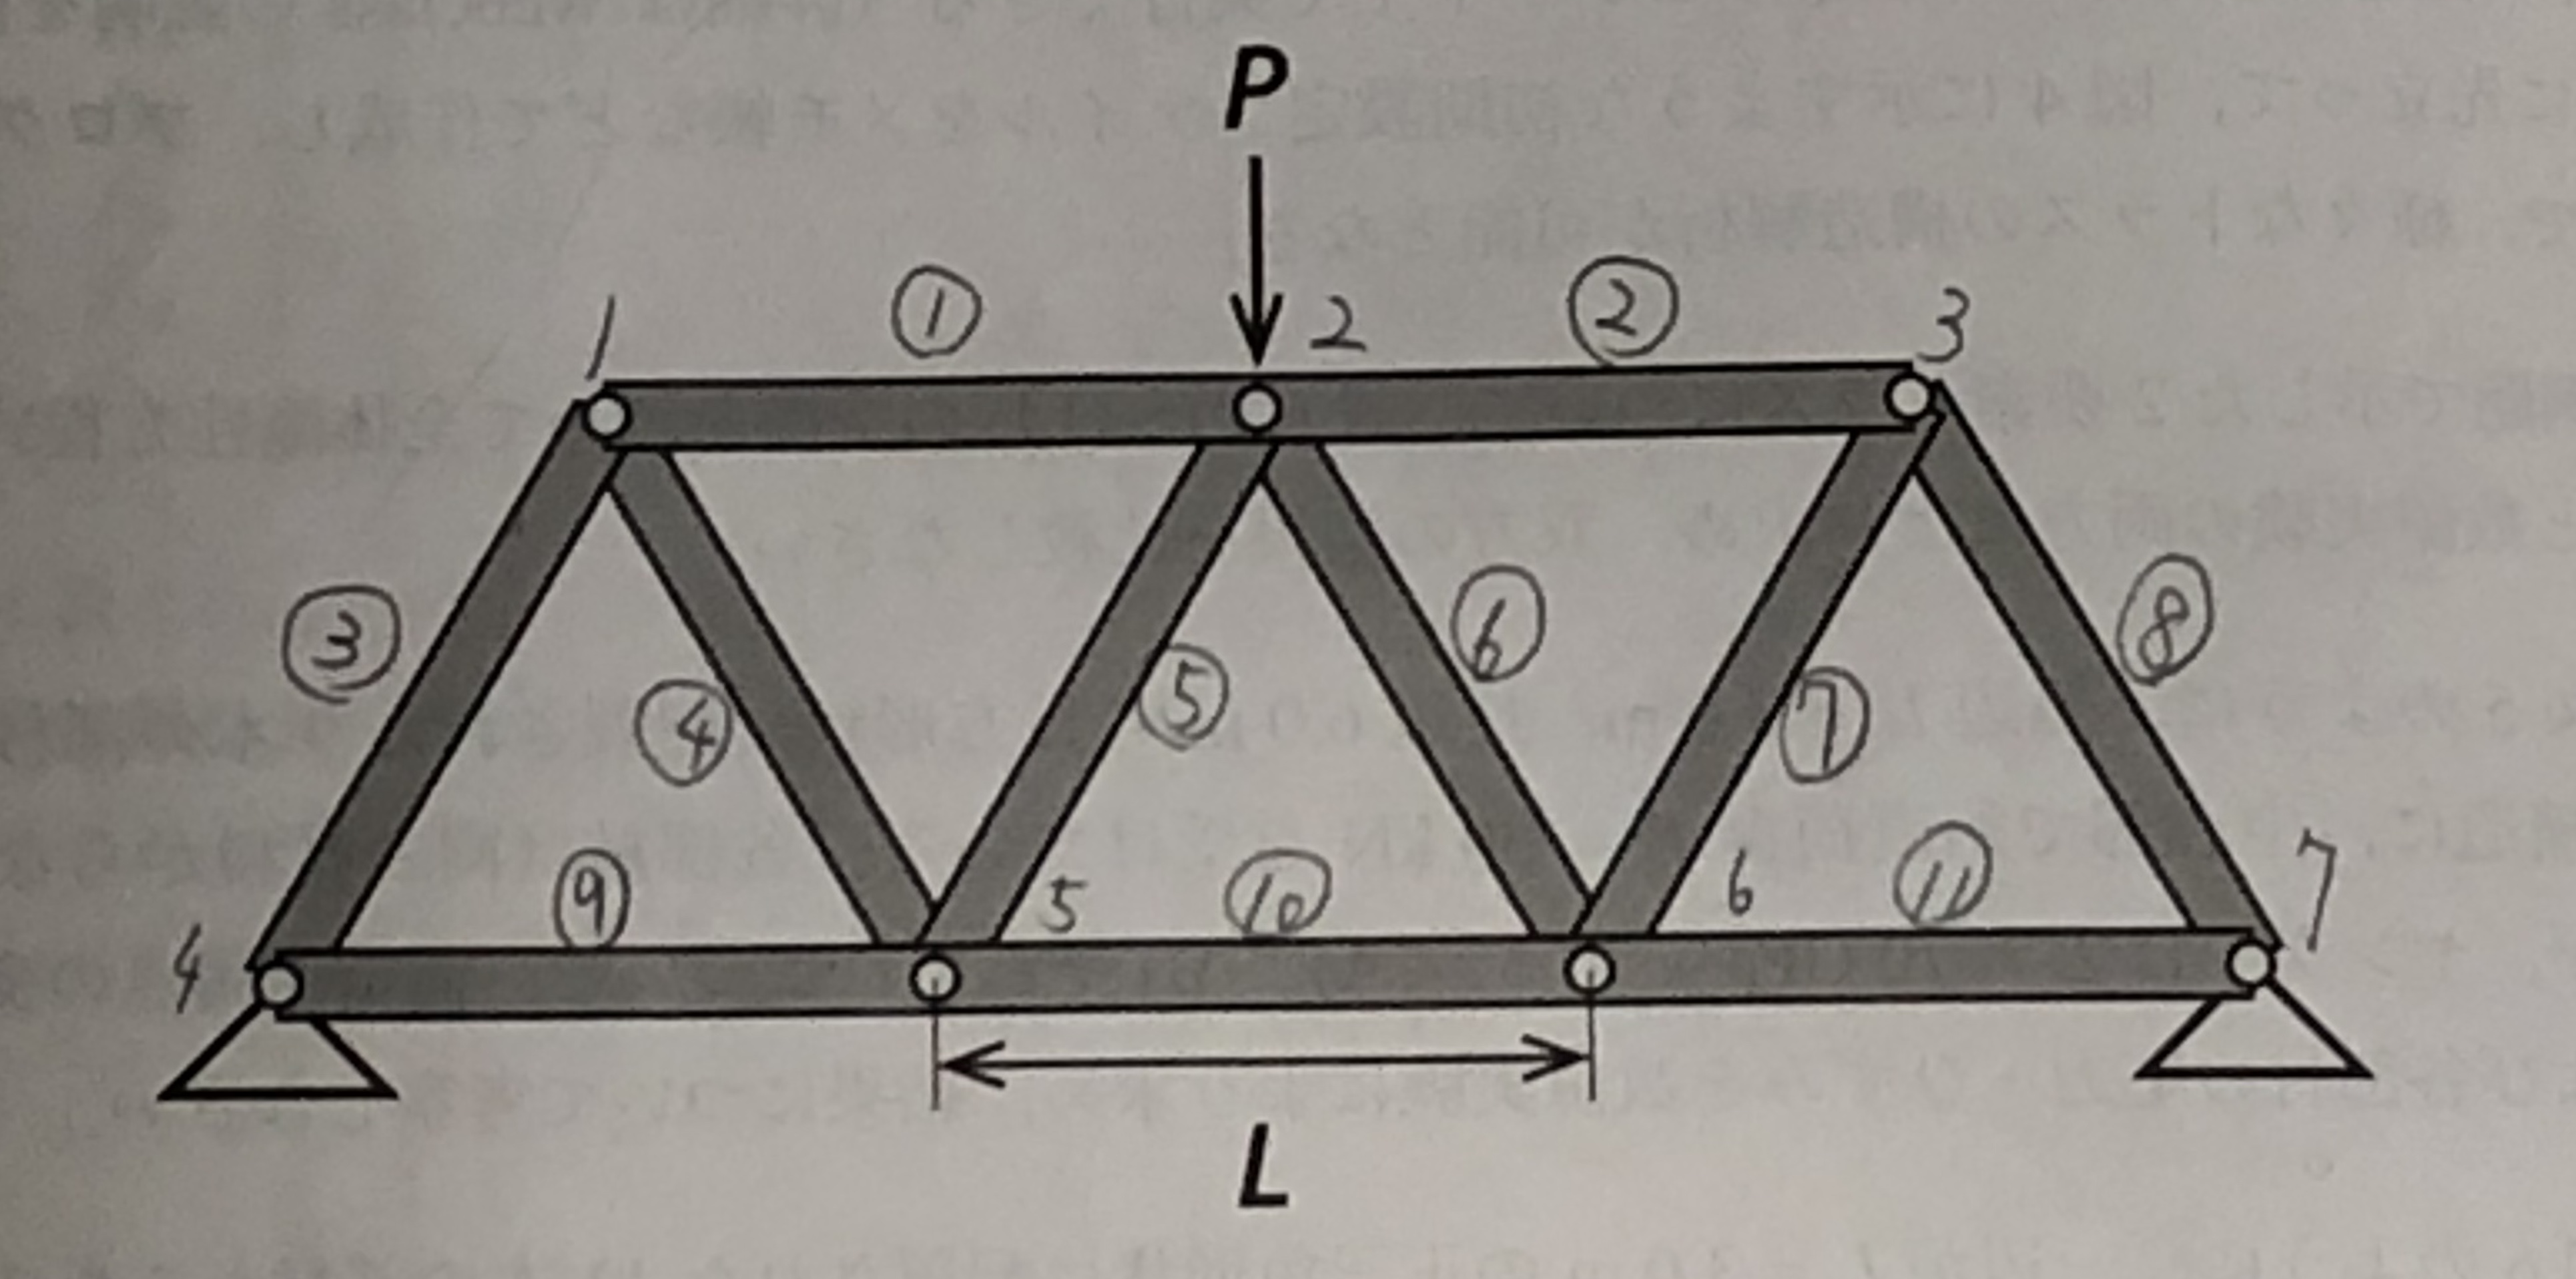
\includegraphics[width = 8cm]{画像/trus_11.JPG}
    \caption{11部材からなるトラス構造}
    \label{truss11}
  \end{center}
\end{figure}

\subsection{平面応力解析}
図\ref{板}のように,半径$a=200$mm の円孔を有する一辺2000mm,厚さ1mmの正方形板について考える.$y = \pm 1000$mmの上辺と下辺を一様な等分布荷重$T=20$MPaで引っ張ったとき,円孔の
周りにどのような力が作用するかを観察した.
解析の方法は以下の通りである.

\begin{figure}[H]
  \begin{center}
    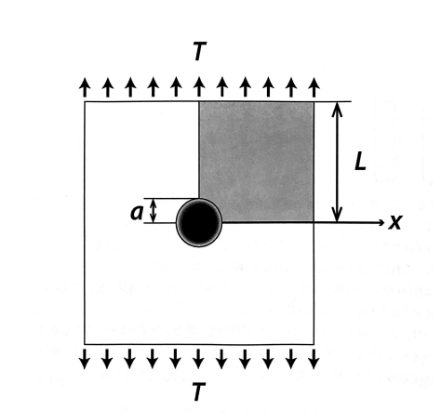
\includegraphics[width = 8cm]{画像/板.png}
    \caption{円孔板の引っ張り}
    \label{板}
  \end{center}
\end{figure}

\begin{description}
  \item[(a)] 解析の対象となる領域を分割し,要素で埋め尽くした.
  \begin{itemize}
    \item なるべく正三角形に近い三角形を用いた
    \item 三角形の辺上にはあらたん節点を作らない.
    \item 応力集中すなわち応力勾配が大きいと予想されるところは細かく分割した.
  \end{itemize}
  \item[(b)] 節点に番号をつけ,節点の($x,y$)座標リストを作成した.
  \begin{itemize}
    \item 1番から順番に番号つけをし,欠番がないようにした.
  \end{itemize}
  \item[(c)]要素に番号をつけ,各要素の3節点を反時計回りになるように列挙した.
  \item[(d)]解析対象を取り囲む外形戦場の節点座標を列挙した.
  \item[(e)]境界条件を設定した.
  \begin{itemize}
    \item 端部の節点に作用する力についての条件を求めた.
    \item 端部の節点の変位についての条件を求めた.
  \end{itemize}
  \item[(f)]材料の力学的特性値(ヤング率,ポアソン比,厚み)を調べ,設定した.
  \item[(g)]以上の条件を応力計算ソフトウェアに入力し,計算した..
\end{description}


\section{実験結果及び考察}
\subsection{課題1}
2トラス構造の計算結果のデータについては付録に添付した.
2トラス構造の解析結果を可視化した図を以下に示す.
\begin{figure}[H]
  \begin{center}
    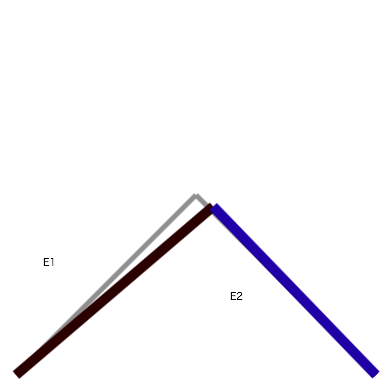
\includegraphics[width = 8cm]{画像/2.png}
    \caption{2トラス構造の解析結果}
    \label{2解析}
  \end{center}
\end{figure}

2トラス構造の各部材に応力と歪みを手計算と数値計算それぞれで求め,以下の表にまとめた.
\begin{table}[H]
\begin{center}
\caption{2トラス構造の歪みと応力}
\begin{tabular}{l|ll}
          & 手計算         & 数値計算        \\ \hline
$\epsilon_a$& $1.767 \times 10^{-4}$ & $1.767 \times 10^{-4}$   \\ \hline
$\epsilon_b$& $-8.838 \times 10{-4}$ & $-8.838 \times 10{-4}$ \\ \hline
$\sigma_a$[MPa]  & 35.355      & 35.355      \\ \hline
$\sigma_b$[MPa]& -176.77     & -176.77
\end{tabular}
\end{center}
\end{table}
応力およびひずみの手計算と数値計算による結果が一致した.4桁,5桁まで見ても一致しており,今回の2トラス実験のスケールにおいては数値解析の精度が高いことが確かめられた.
手計算による方法では時間がかかる上,パラメータを変化させるごとに計算し直さなくてはならない,また計算を間違える恐れがあるが,
数値解析では一度実装してしまえばパラメータを入力し直すことで何度でもすぐに計算でき,有用であると考える.
しかしながら,正しい実装を行えていない場合や,実装が解析対象に対応し切れていない可能性もあるため,
手計算によって正しい計算結果と精度を確認することも構造解析において重要であると言える.

\subsection{課題2}
9部材からなるトラス構造の計算結果のデータについては付録に添付した.
9部材からなるトラス構造の解析結果を可視化した図を以下に示す.

\begin{figure}[H]
  \begin{tabular}{cc}
    \begin{minipage}{0.5\hsize}
      \begin{center}
        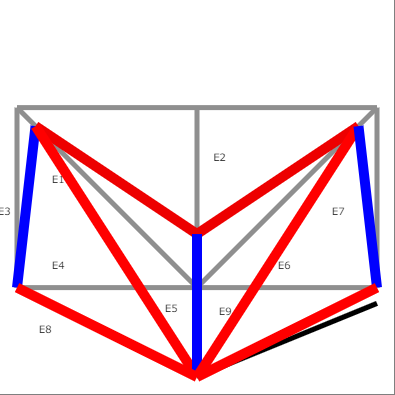
\includegraphics[width = 5cm]{画像/A.png}
        \caption{9部材からなるトラス構造の解析結果(A)}
        \label{9解析A}
      \end{center}
    \end{minipage}

    \begin{minipage}{0.5\hsize}
      \begin{center}
        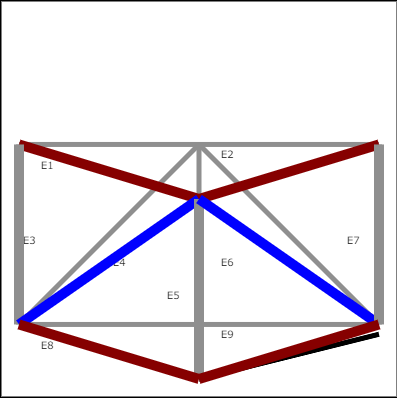
\includegraphics[width = 5cm]{画像/B.png}
        \caption{9部材からなるトラス構造の解析結果(B)}
        \label{9解析}
      \end{center}
    \end{minipage}
  \end{tabular}
\end{figure}

\begin{description}
  \item[(A)]上下の平行な要素と正方形の対角要素に強い引っ張り応力がかかっていることがわかる.
  また,縦の3つの要素には圧縮応力がかかっており,大きくたわんでしまっていることがわかる.
  これは荷重をかけた中心の要素を左右の縦の要素3,7が自由点を支点に釣り上げるような構造になっているため,
  荷重に対して引っ張り方向に支える要素が圧縮方向に支える要素よりも多くなり,耐え切れなくなっていると考えられる.

  \item[(B)]上下の平行な要素に小さな引っ張り応力がかかっており,正方形の対角要素に圧縮応力がかかっていることがわかる.
  また縦の3つの要素にはほとんど応力がかかっていないことがわかる.この構造では縦の3要素と対角線の2要素が圧縮方向に荷重を支えており,
  上下の4要素が引っ張り方向に支えているため,要素にかかる応力及び歪みが小さくなっていると考えられる.

\end{description}

\subsection{課題3}
11部材からなるトラス構造の計算結果のデータについては付録に添付した.
11部材からなるトラス構造の解析結果を可視化した図を以下に示す.

\begin{figure}[H]
  \begin{center}
    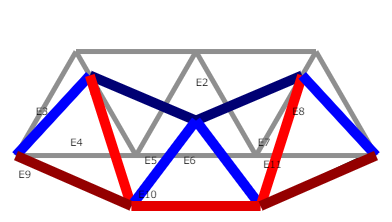
\includegraphics[width = 10cm]{画像/11.png}
    \caption{11部材からなるトラス構造の解析結果}
    \label{11解析}
  \end{center}
\end{figure}


要素1,2にはわずかな圧縮応力がかかっており,要素3,5,6,8にはおよそ等しく圧縮応力がかかっている.
また,要素4,7,10には強い引っ張り応力がかかっており,9,11にはわずかな引っ張り応力がかることがわかった.
9部材のトラス構造について考えたように圧縮方向の部材と引っ張り方向の要素を比較すると,圧縮は5要素,引っ張りは6要素となっており,
引っ張り要素の方が多い.つまり課題2のAの構造に近いと言える.課題2での考えが正しいとすれば,この構造において
要素4,7をそれぞれ90度回転させ,節と接合すると,部材の$L$は変わってしまうが,よりたわみの小さい構造になるのではないかと考えられる.

\subsection{課題4}
有限要素解析を行うにあたり準備した節点表,要素表,外形表及び,円孔と$x$軸に隣接する要素の応力表は付録に添付した.
有限要素分割図,$x$方向応力,$y$方向応力,せん断方向応力の可視化図を以下に示す.

\begin{figure}[H]
  \begin{center}
    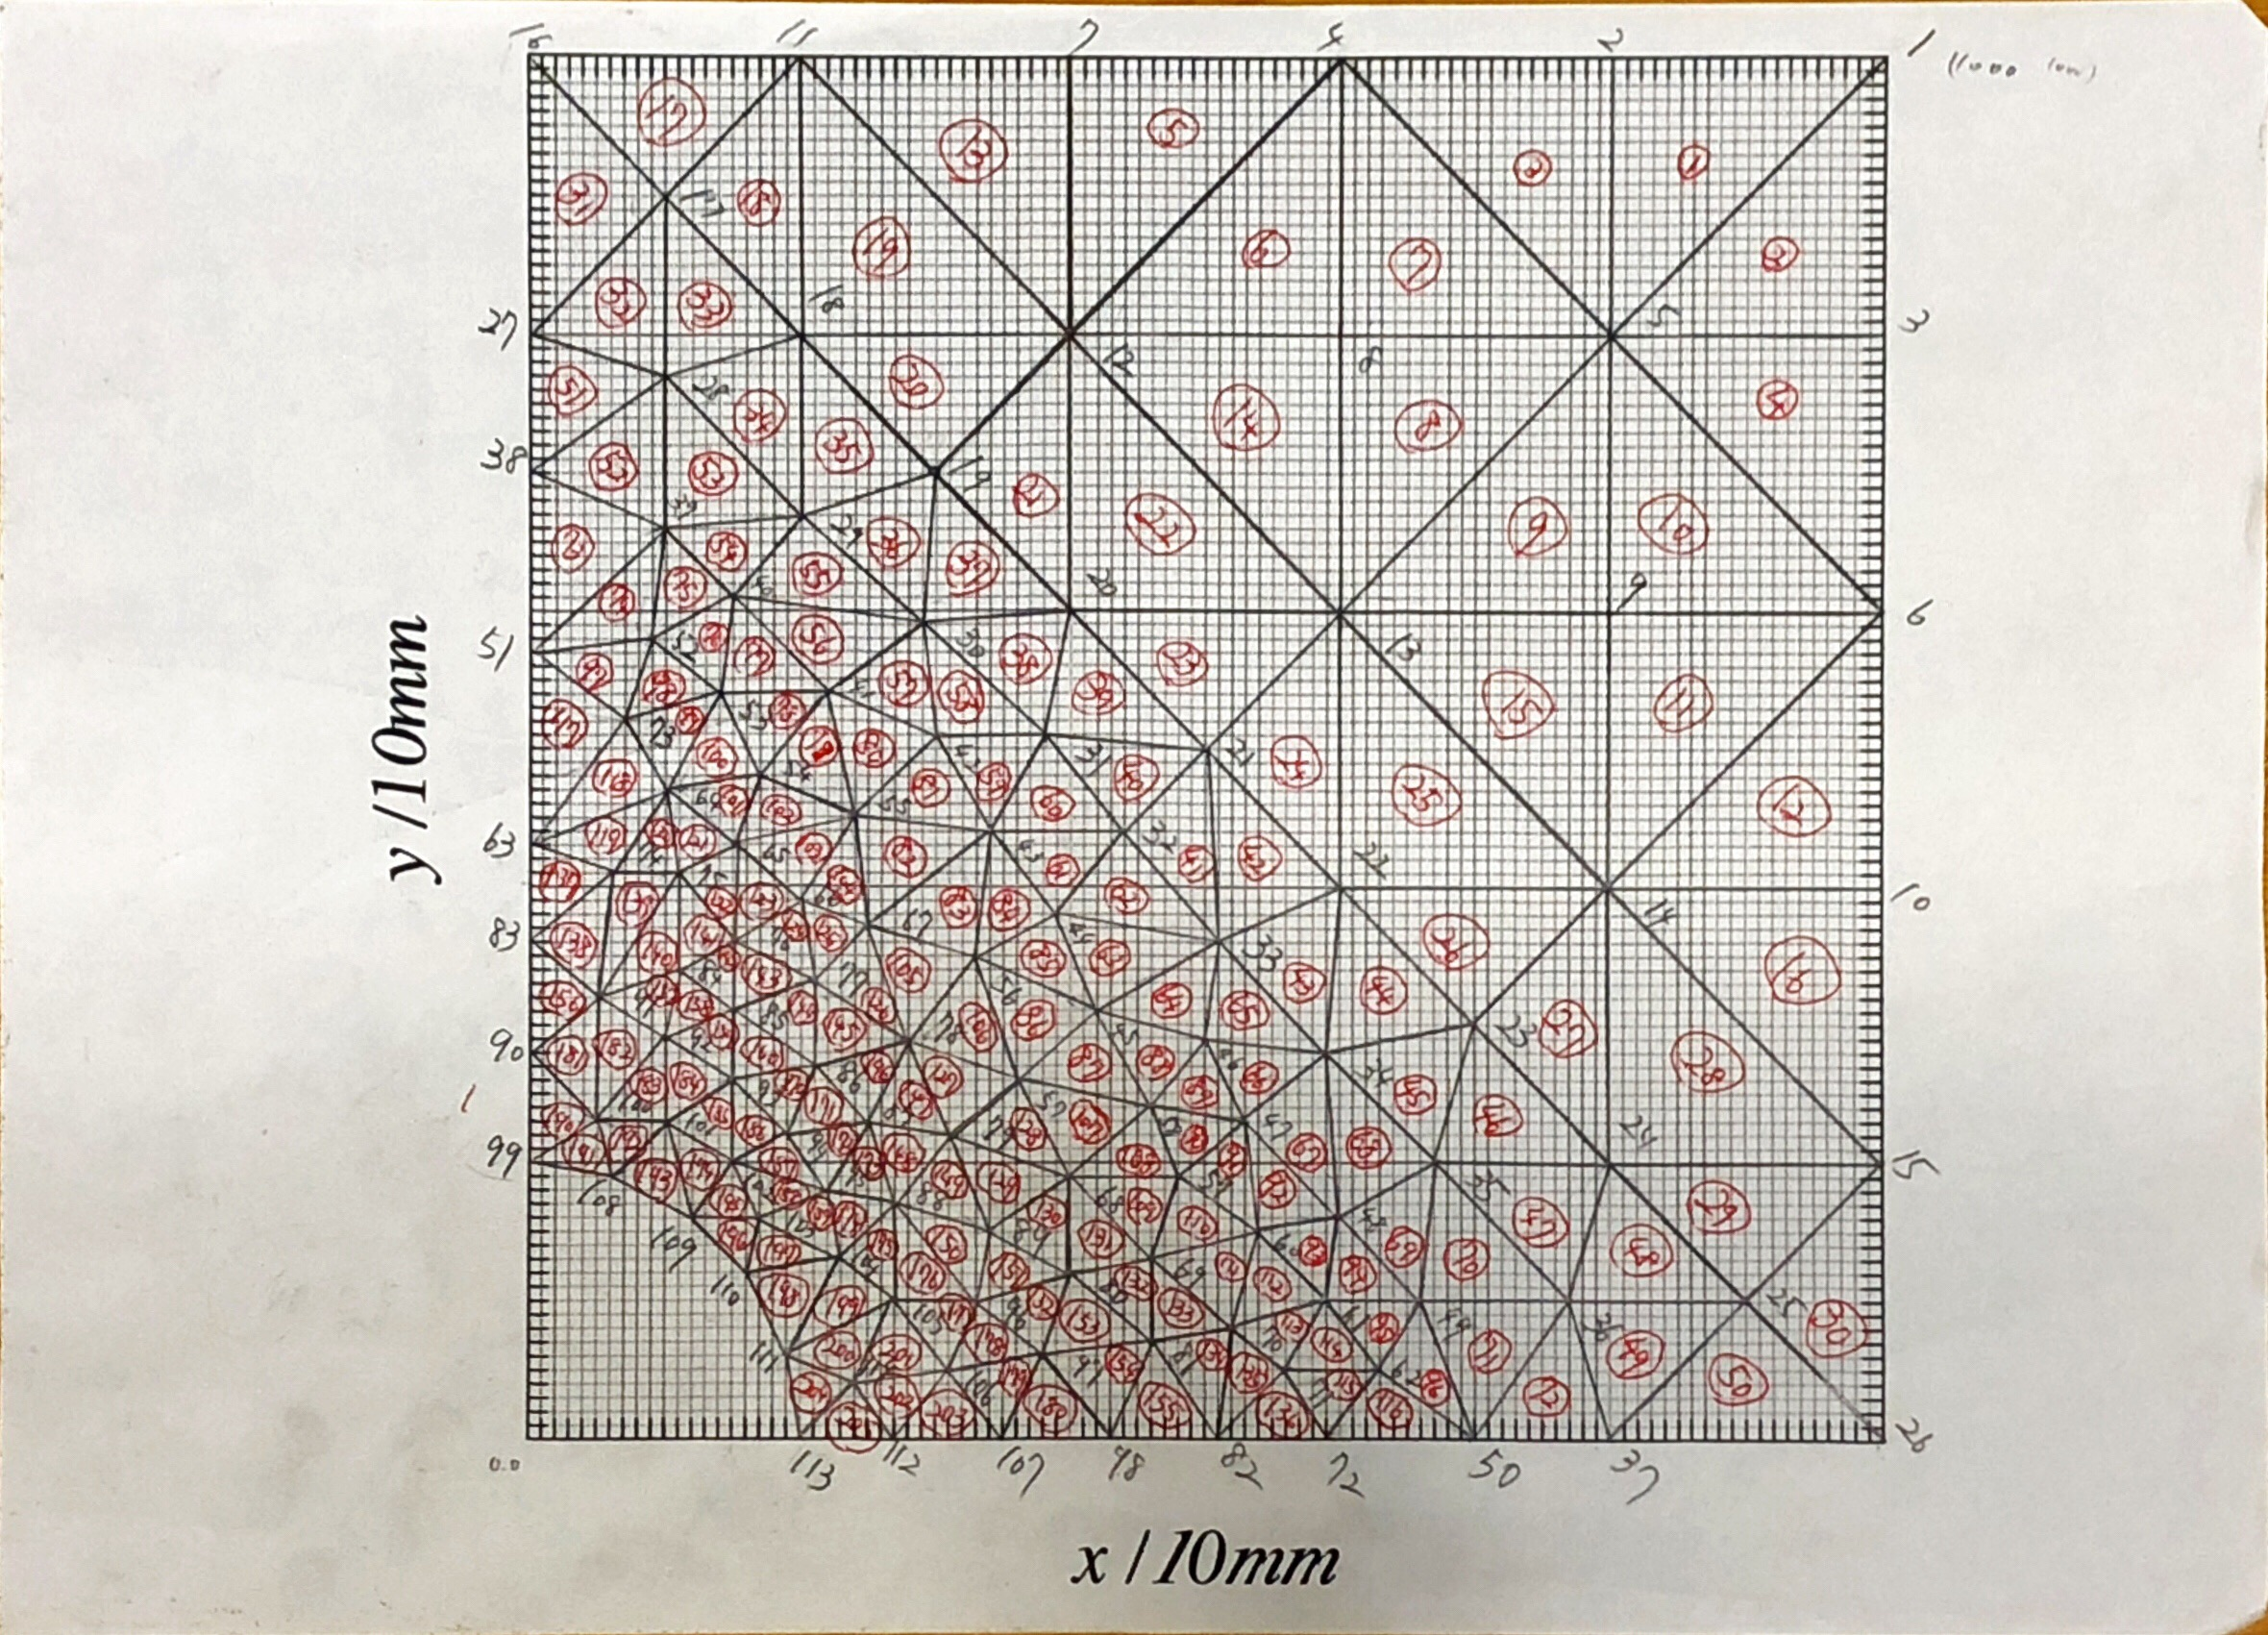
\includegraphics[width = 10cm]{画像/youso.jpg}
    \caption{有限要素分割図}
    \label{有限要素分割図}
  \end{center}
\end{figure}

\begin{figure}[H]
  \begin{tabular}{cc}
    \begin{minipage}{0.5\hsize}
      \begin{center}
        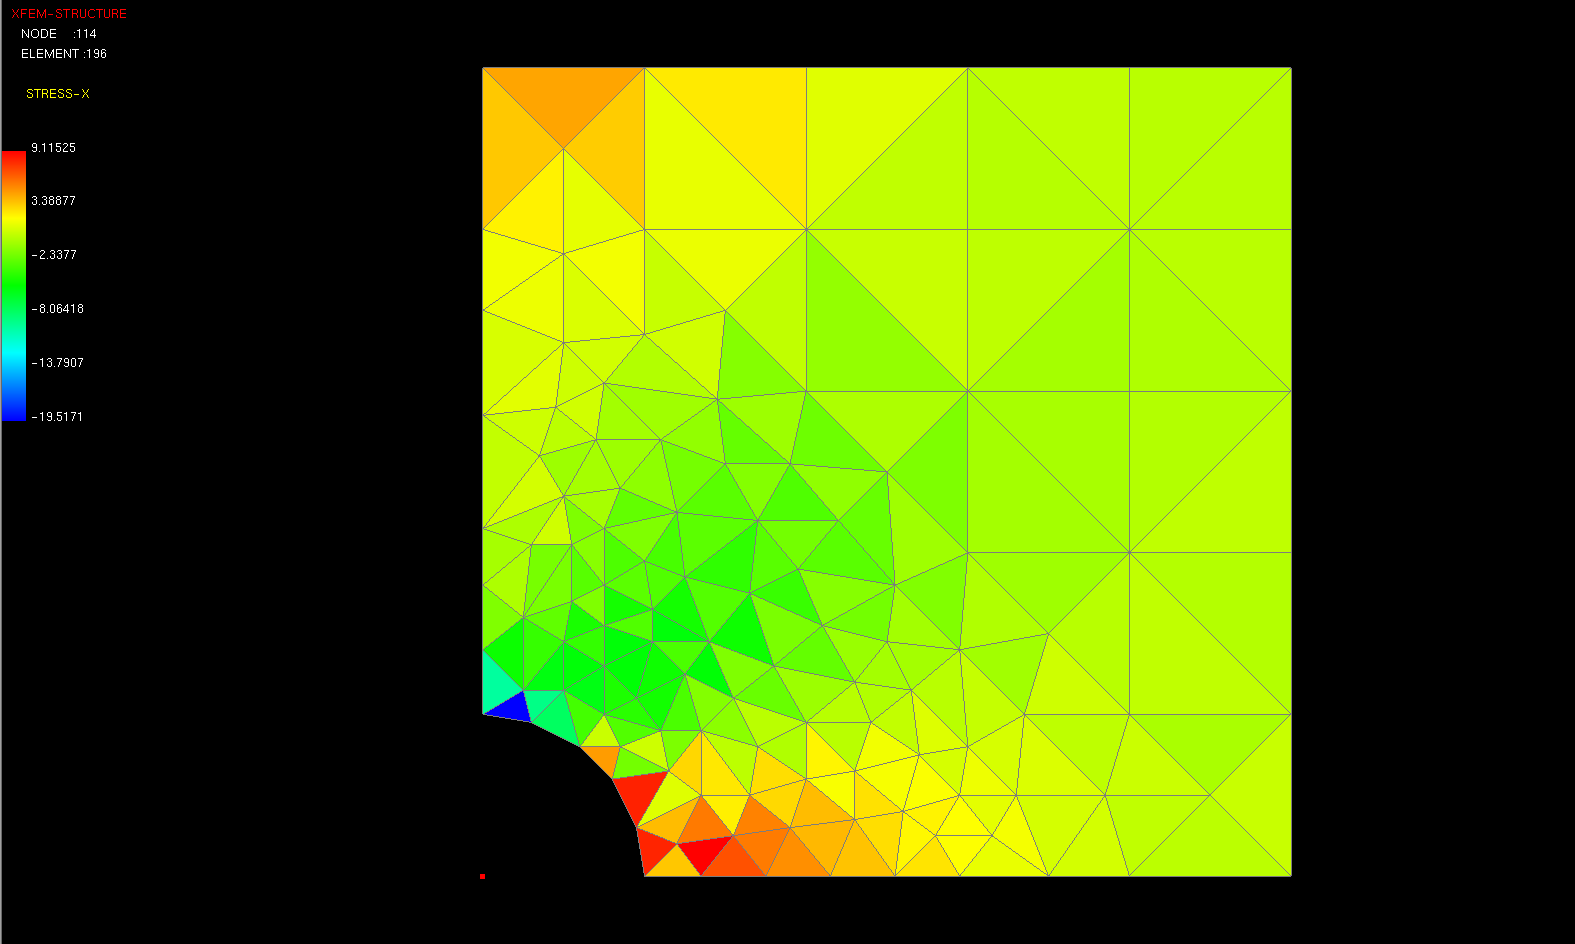
\includegraphics[width = 5cm]{画像/x_1.png}
        \caption{$\sigma_x$分布図(変位倍率:1倍)}
        \label{x_1}
      \end{center}
    \end{minipage}

    \begin{minipage}{0.5\hsize}
      \begin{center}
        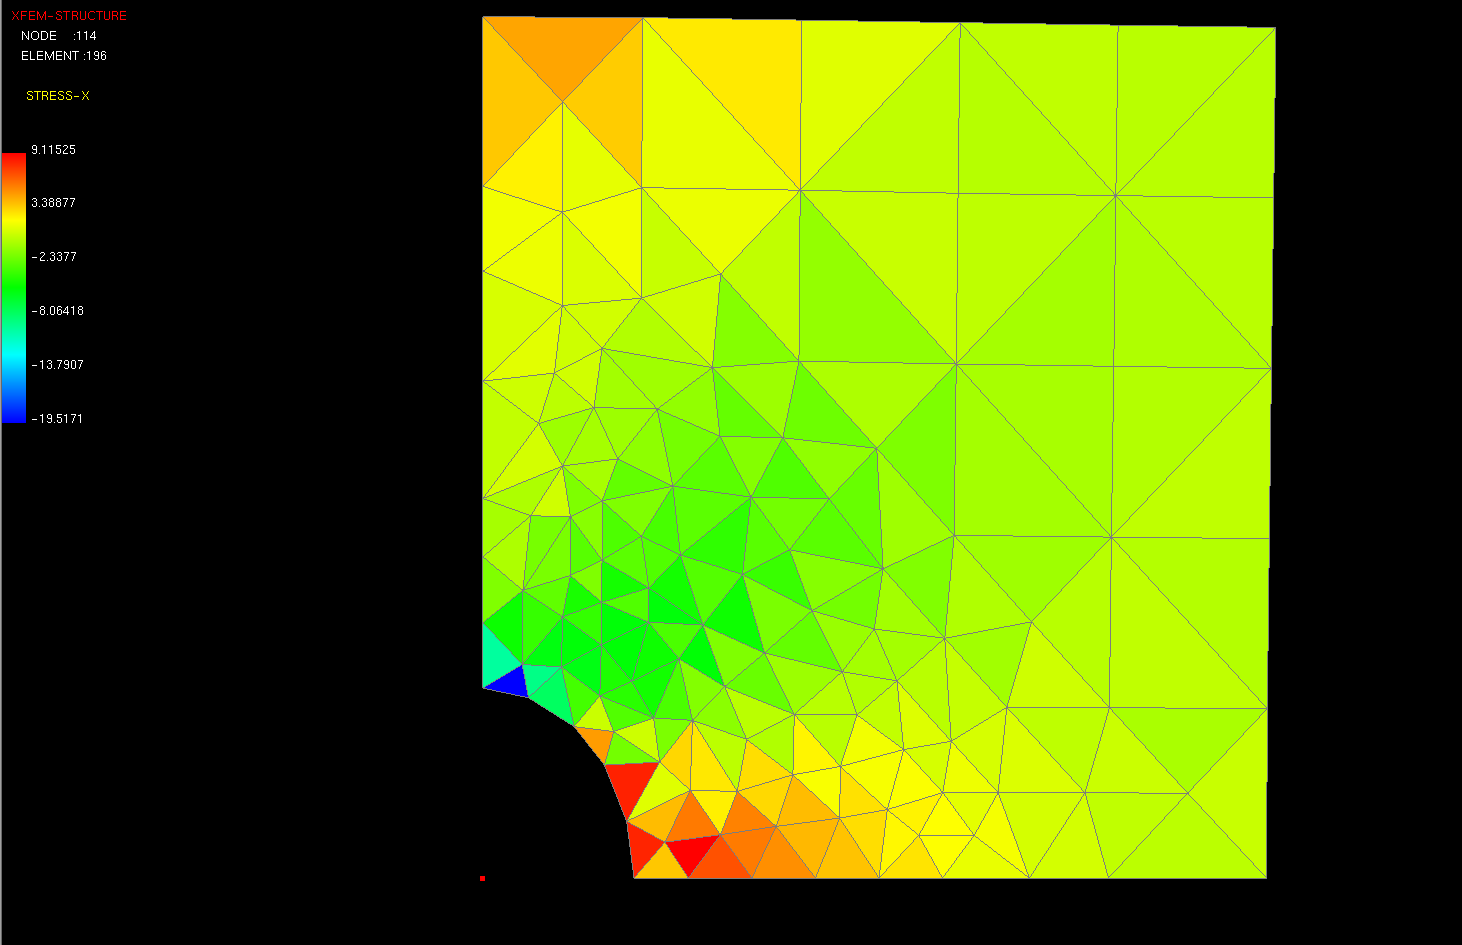
\includegraphics[width = 5cm]{画像/x_600.png}
        \caption{$\sigma_x$分布図(変位倍率:600倍)}
        \label{x_600}
      \end{center}
    \end{minipage}
  \end{tabular}
\end{figure}

\begin{figure}[H]
  \begin{tabular}{cc}
    \begin{minipage}{0.5\hsize}
      \begin{center}
        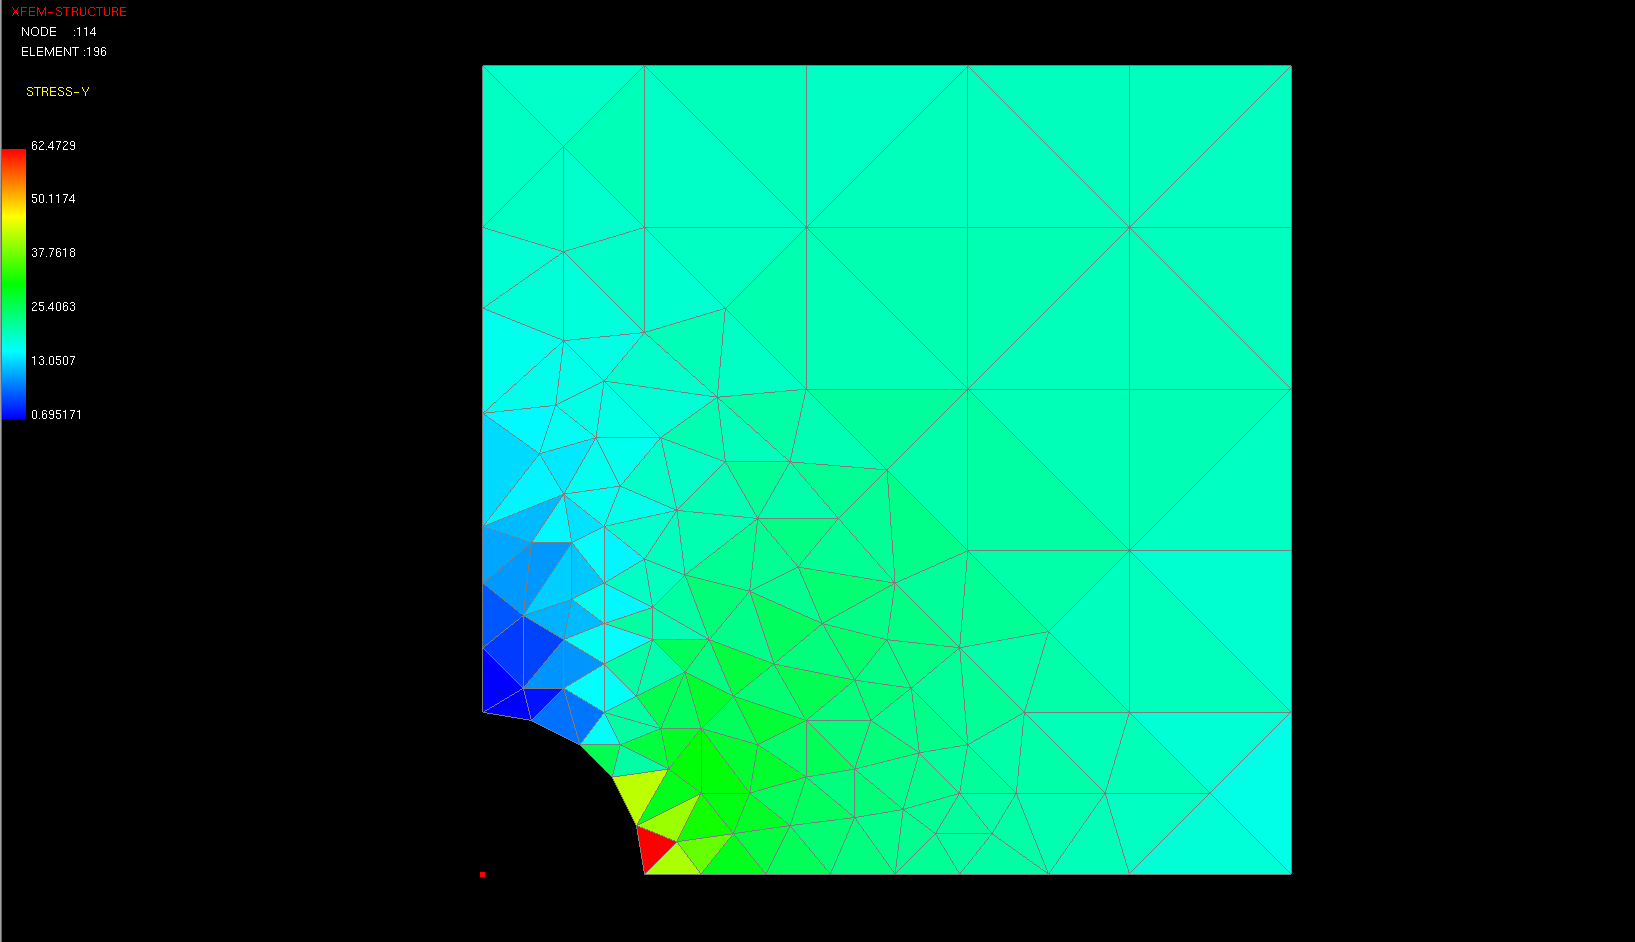
\includegraphics[width = 5cm]{画像/y_1.png}
        \caption{$\sigma_y$分布図(変位倍率:1倍)}
        \label{y_1}
      \end{center}
    \end{minipage}

    \begin{minipage}{0.5\hsize}
      \begin{center}
        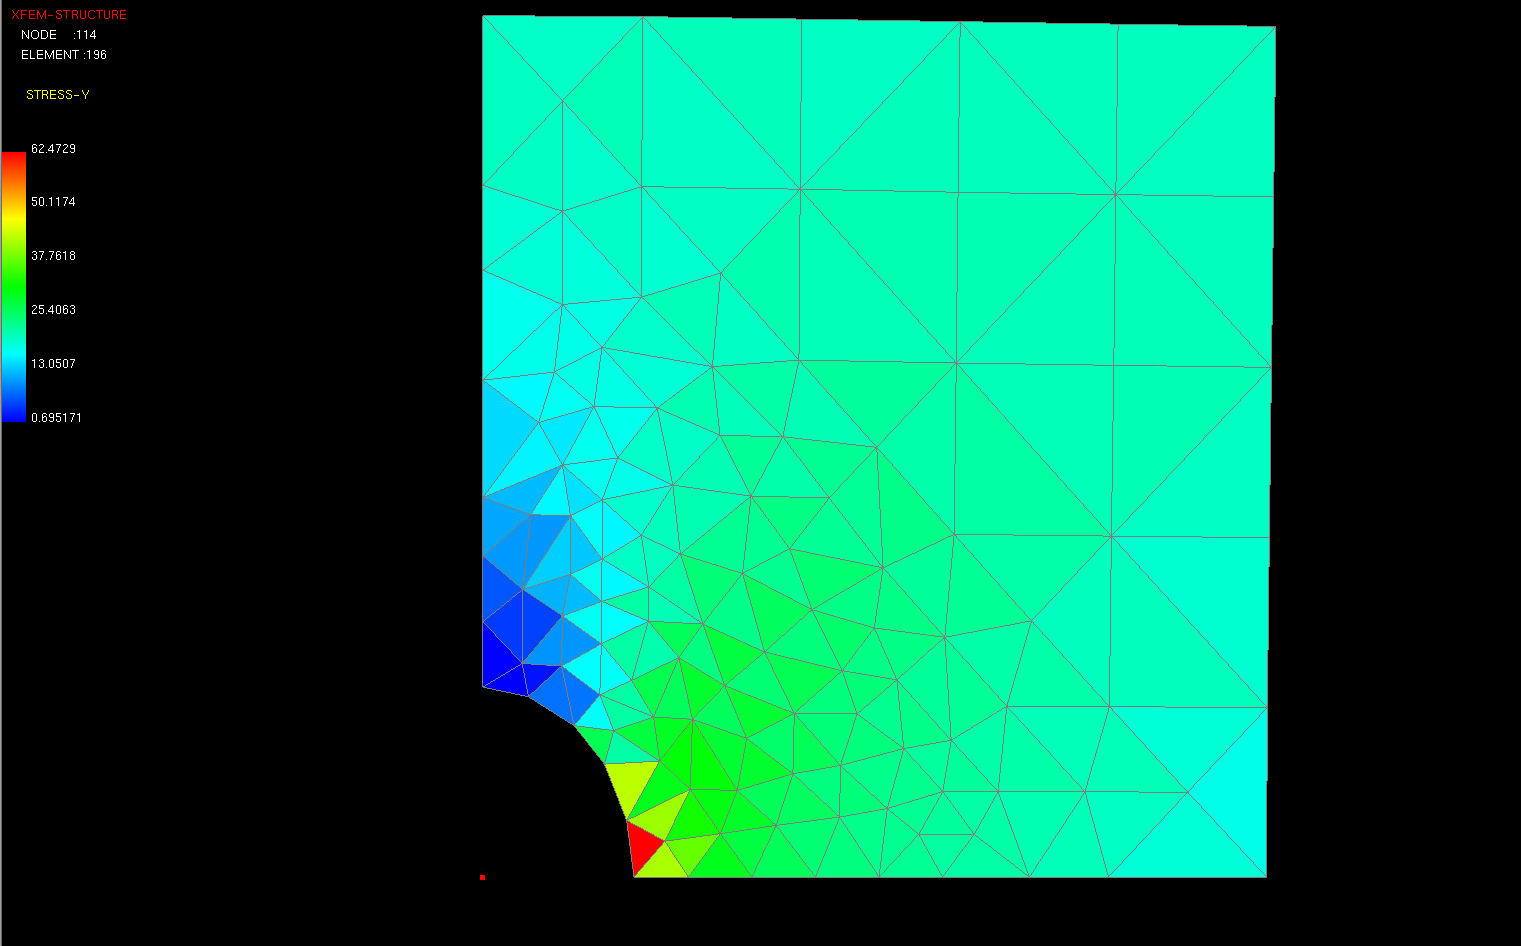
\includegraphics[width = 5cm]{画像/y_600.png}
        \caption{$\sigma_y$分布図(変位倍率:600倍)}
        \label{y_600}
      \end{center}
    \end{minipage}
  \end{tabular}
\end{figure}

\begin{figure}[H]
  \begin{tabular}{cc}
    \begin{minipage}{0.5\hsize}
      \begin{center}
        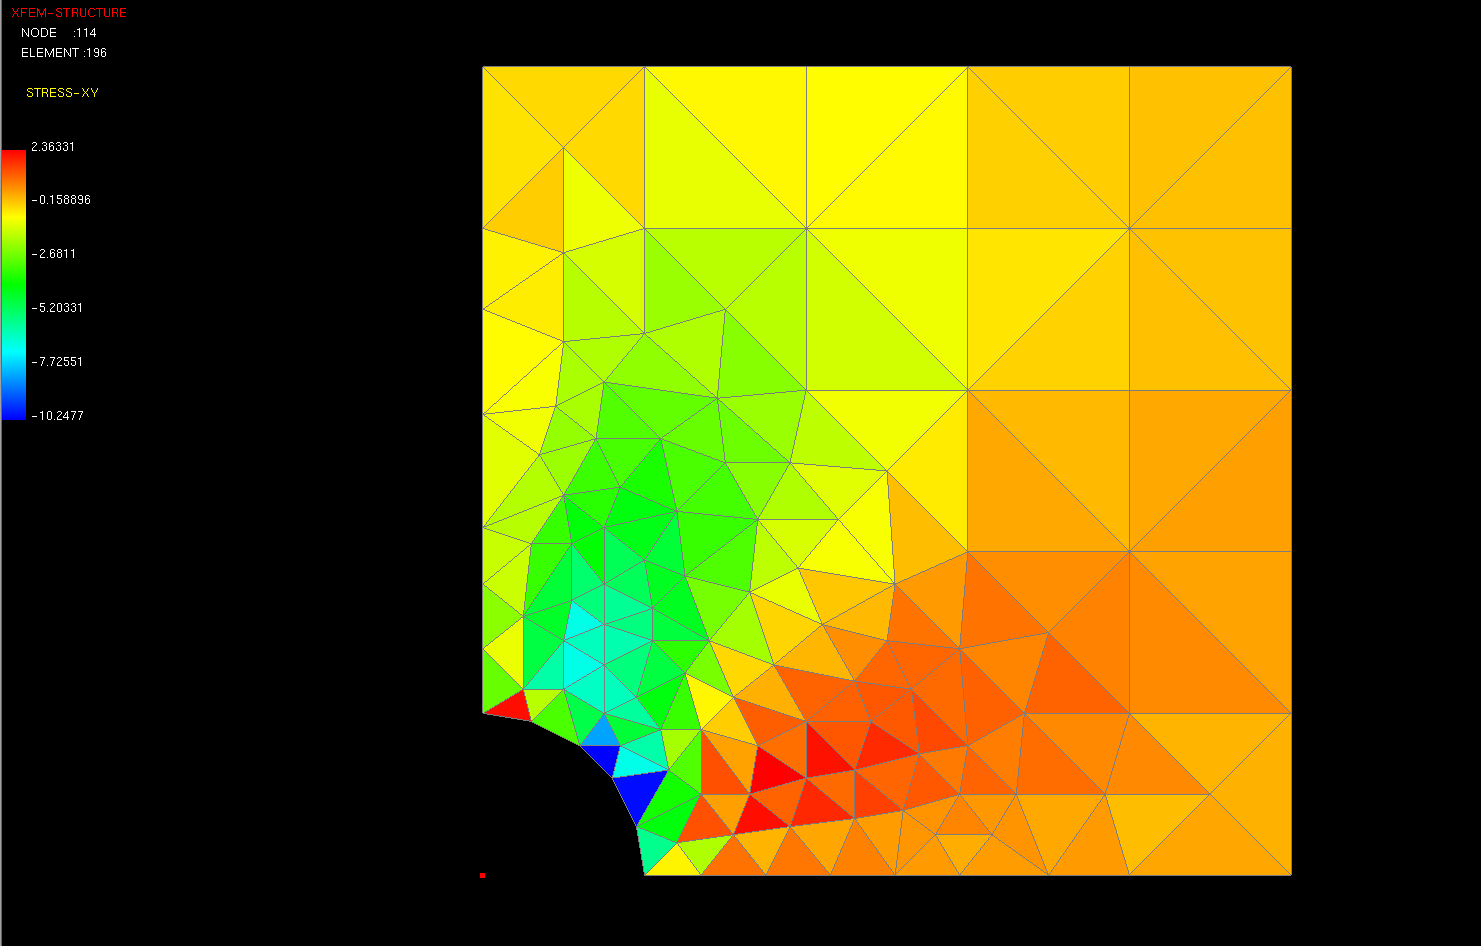
\includegraphics[width = 5cm]{画像/xy_1.png}
        \caption{$\sigma_xy$分布図(変位変位倍率:1倍)}
        \label{xy_1}
      \end{center}
    \end{minipage}

    \begin{minipage}{0.5\hsize}
      \begin{center}
        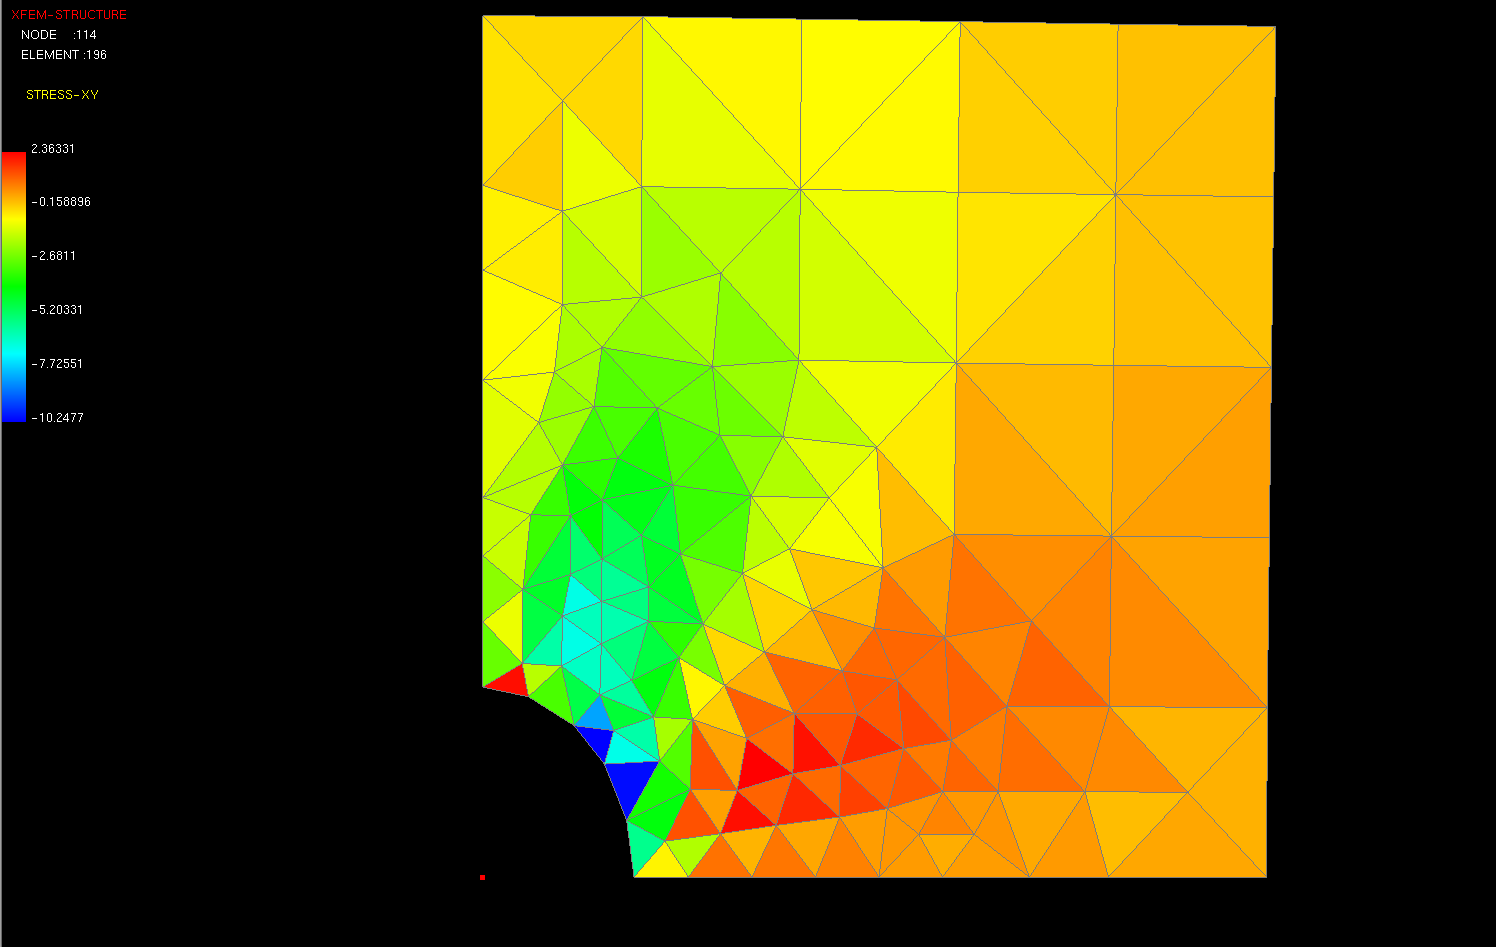
\includegraphics[width = 5cm]{画像/xy_600.png}
        \caption{$\sigma_xy$分布図(変位倍率:600倍)}
        \label{xy_600}
      \end{center}
    \end{minipage}
  \end{tabular}
\end{figure}

また、円弧の周りおよび$x$軸上の要素における$\sigma_x$および$\sigma_y$の解析結果を次の表に示した。

\begin{table}[H]
\begin{center}
\begin{tabular}{lll|lll}
円孔 &  &  & $x$軸 &  &  \\
要素番号 & $\sigma_x$ & $\sigma_y$ & 要素番号 & $\sigma_x$ & $\sigma_y$ \\ \hline
181 & -19.5171 & 0.695171 & 195 & 3.53049 & 41.9159 \\ \hline
183 & -7.88984 & 7.64884 & 193 & 6.85755 & 29.9016 \\ \hline
186 & 4.74593 & 26.6745 & 170 & 5.10502 & 26.307 \\ \hline
188 & 8.2146 & 43.0094 & 155 & 3.65724 & 23.9977 \\ \hline
194 & 8.10598 & 62.4729 & 136 & 2.7314 & 22.6035 \\ \hline
 &  &  & 116 & 1.36352 & 21.607 \\ \cline{4-6}
 &  &  & 72 & 0.741738 & 20.4293 \\ \cline{4-6}
 &  &  & 50 & 0.00637526 & 18.6505
\end{tabular}
\end{center}
\end{table}

分布図を見ると,$\sigma_x,\sigma_y$の両方とも,円孔の周りでは$y$軸近くで圧縮応力が発生し,$x$軸に近づくにつれて引っ張り応力が大きくなっていることがわかる.
$\sigma_x$では円孔に隣接した要素に加え,円孔付近の$x$軸の近傍でも強い引っ張り応力が見られる.
しかし,$\sigma_y$では円孔に隣接した要素にしか引っ張り応力が見られない.
これは$y$方向に引っ張り荷重をかけているため,$y$方向に伸びようとする板を$x$方向に伸びることによって荷重を分散させていると思われる.
以上から,このようなモデルの設計をする際には円孔の$x$軸付近の強度を強くする必要があることがわかった.

\par
無限平板に対する引っ張り応力$\sigma_y$の解析解は,$x$軸に接している要素重心の$x$座標に対して
\begin{align}
  \sigma_y = \frac{T}{2} \left(1+ \left(\frac{a}{x}\right)^2 + \left(1 + 3\left(\frac{a}{x}\right)^4\right)\right)
\end{align}
のように表される.ただし,$T$は上下辺を加えた応力,$a$は円孔半径,$x$は$x$軸上の位置である.
数値解析で得られた$x$軸に接している要素の重心の座標$x$を横軸に,その要素の$y$方向応力$\sigma_y$
を縦軸とするグラフに解析解をプロットしたグラフを以下に示す.
\begin{figure}[H]
  \begin{center}
    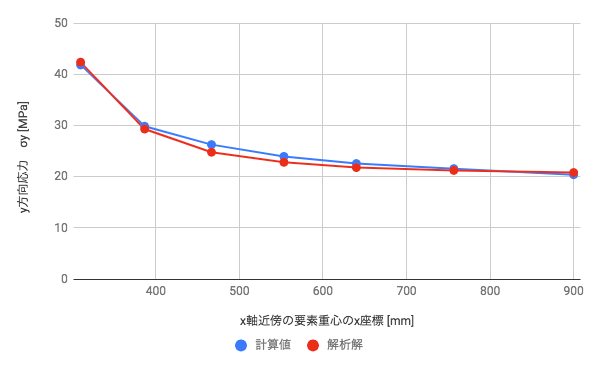
\includegraphics[width = 10cm]{画像/グラフ.png}
    \caption{$x$軸上の要素の$\sigma_y$の計算値と解析値の比較}
    \label{比較}
  \end{center}
\end{figure}

計算値と解析値を比較すると,概ね沿っているが,重心の$x$座標が470mm〜750mmの範囲で計算値が解析値を上回っていることがわかる.
図\ref{有限要素分割図}を確認すると,当該範囲での要素が鋭角を含む二等辺三角形のようになっており,正三角形から離れてしまっていることから,
計算値が解析解よりも大きくなってしまったと考えられる.
また,重心の$x$座標が約830mm以降で計算値が解析値を下回っていることについては,解析解によってモデル化できる範囲を超えてしまったためと思われる.
計算値では,900mmにおいて,$\sigma_y$は18.650[MPa]となっており,20[MPa]を下回っている.一方,理論解では,$x$を無限遠に発散させても,20[MPa]が下限である.
つまり,$\sigma_y$が板にかけられた等分布荷重を下回るような点においてはこの解析解ではモデル化し,示すことができないと考えられる.


\subsection{課題5}
授業や,流体の勉強をしていて,有限要素法の名前をよく見てはいたが,実際にどのような手順を踏んでどのような結果が得られるというのはあまり知らなかったので
非常に興味深かった.今回の実験を通して,応力の解析の仕方を理解したが,実際にはこの解析結果を用いて構造的欠陥を発見したり,設計開発へと落とし込んでいく
プロセスが必要になるので今後学んで行きたい.

\section{結論}
いくつかのトラス構造の解析及び円孔板の引張り解析を通して,応力解析の解析手法を理解した.
今回の実験の目的であった,有限要素法における入門的な知識を得るという目標は達成されたと言える.

\section{付録}
\begin{figure}[H]
  \begin{center}
    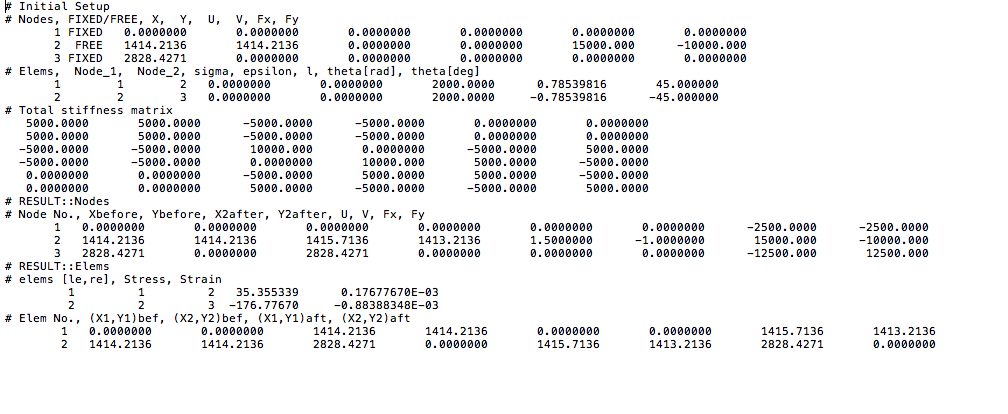
\includegraphics[width = 14cm]{画像/2result.png}
    \caption{2トラス構造の計算結果}
    \label{2解析}
  \end{center}
\end{figure}

\begin{figure}[H]
  \begin{center}
    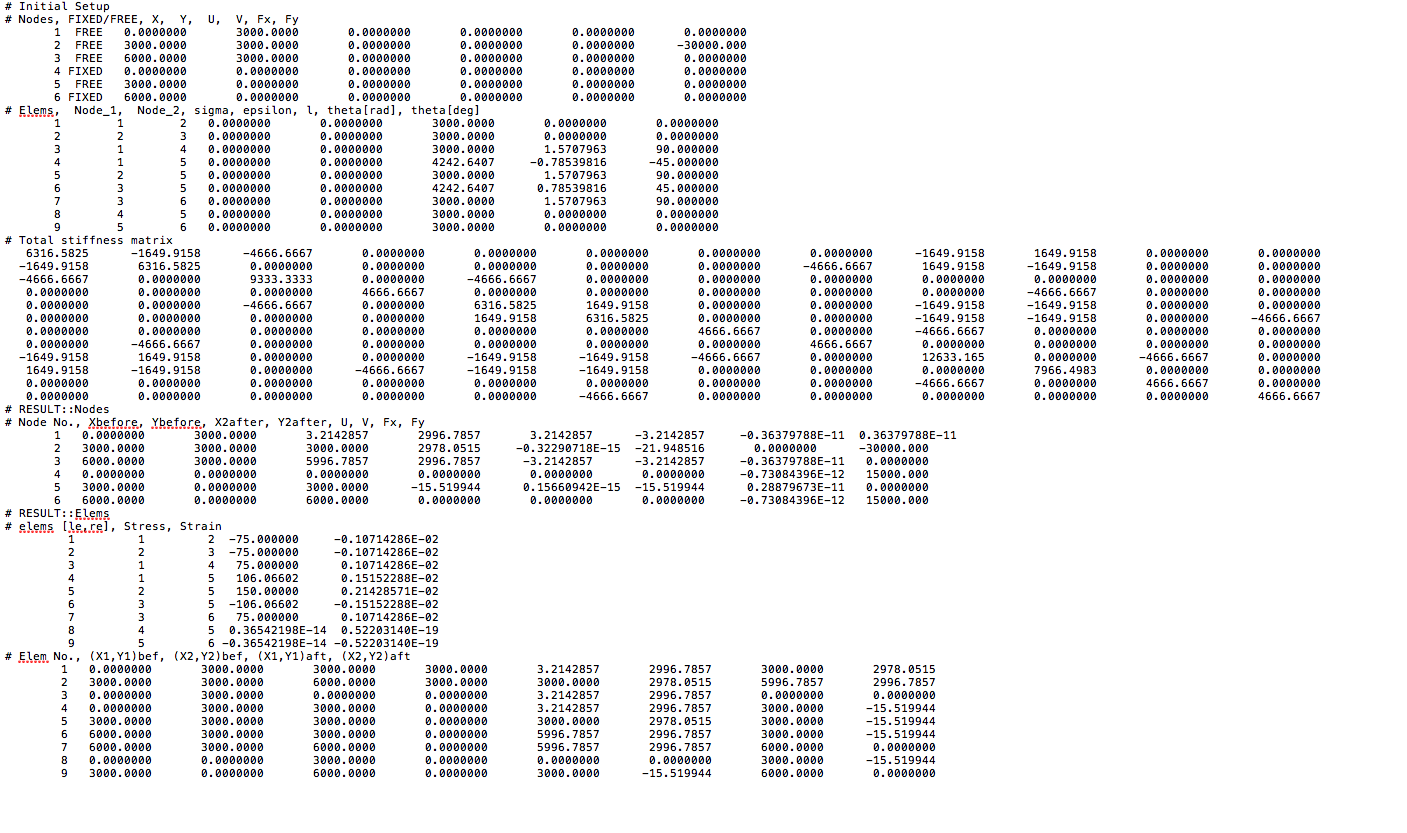
\includegraphics[width = 14cm]{画像/9a.png}
    \caption{9部材からなるトラス構造の計算結果(A)}
    \label{9部材結果A}
  \end{center}
\end{figure}

\begin{figure}[H]
  \begin{center}
    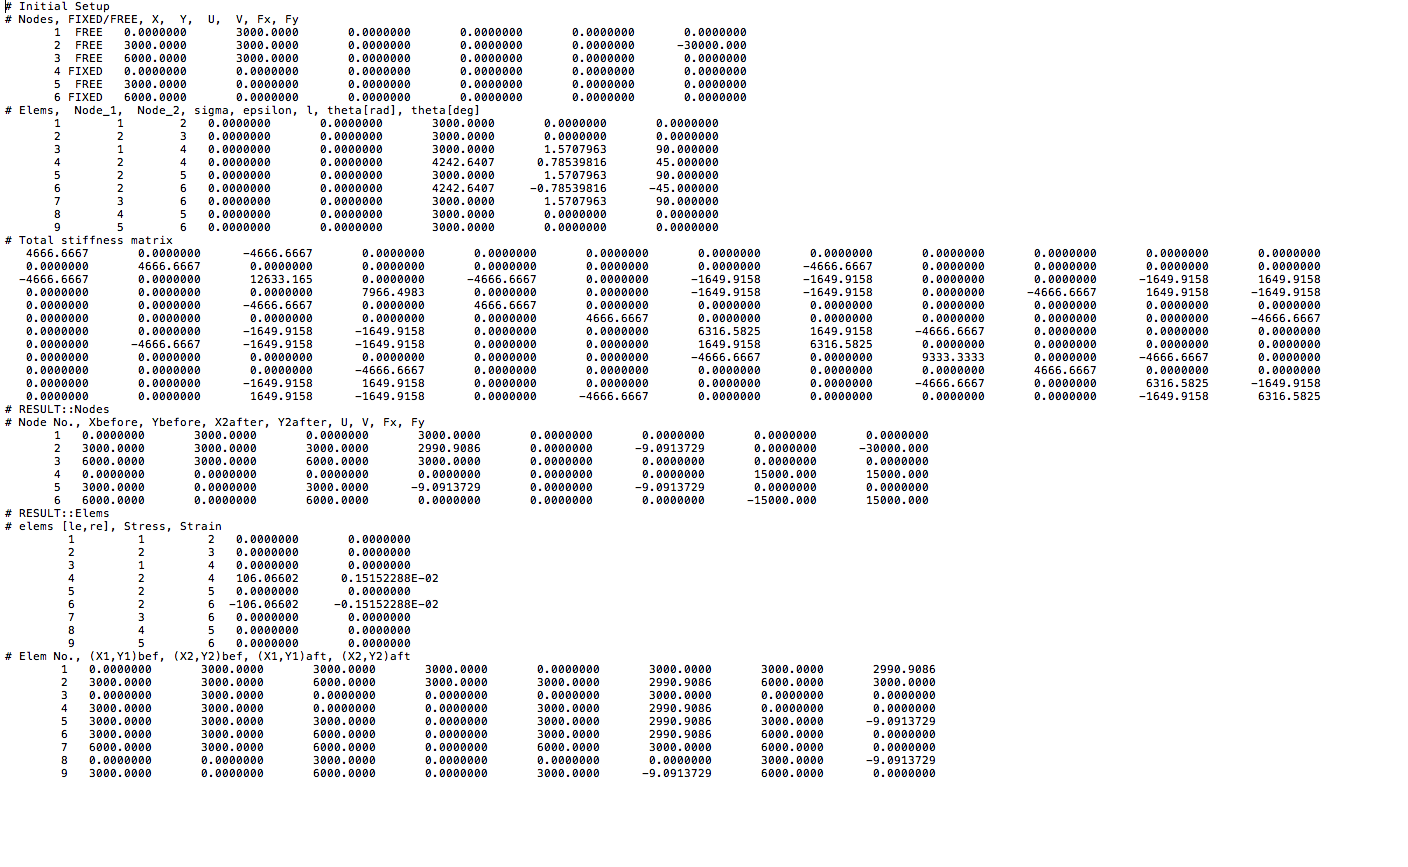
\includegraphics[width = 14cm]{画像/9b.png}
    \caption{9部材からなるトラス構造の計算結果(B)}
    \label{9部材結果B}
  \end{center}
\end{figure}

\begin{figure}[H]
  \begin{center}
    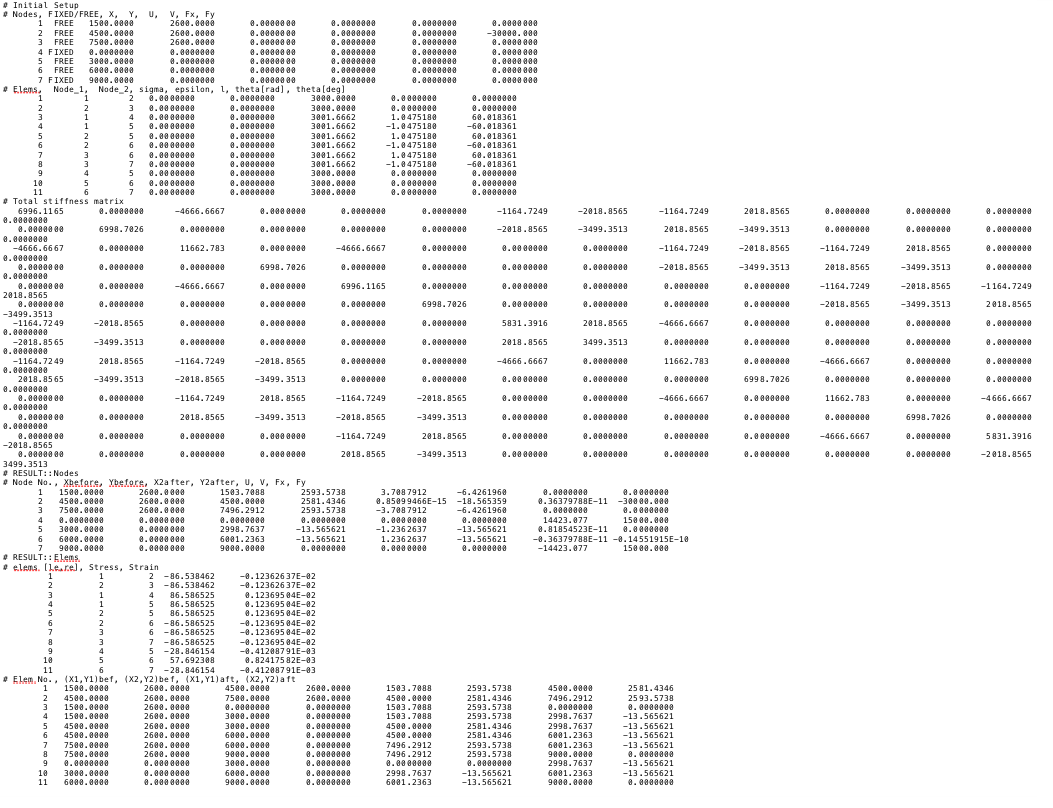
\includegraphics[width = 14cm]{画像/11result.png}
    \caption{11部材からなるトラス構造の計算結果}
    \label{11部材結果}
  \end{center}
\end{figure}

\begin{verbatim}
  節点表
  114
1	1000	1000   
2	800	1000
3	1000	800
4	600	1000
5	800	800
6	1000	600
7	400	1000
8	600	800
9	800	600
10	1000	400
11	200	1000
12	400	800
13	600	600
14	800	400
15	1000	200
16	0	1000
17	100	900
18	200	800
19	300	700
20	400	600
21	500	500
22	600	400
23	700	300
24	800	200
25	900	100
26	1000	0
27	0	800
28	100	770
29	200	670
30	290	590
31	380	510
32	440	440
33	510	360
34	590	280
35	670	200
36	770	100
37	800	0
38	0	700
39	100	660

81	460	70
82	510	0
83	0	360
84	110	340
85	150	310
86	210	290
87	250	250
88	270	180
89	340	160
90	0	280
91	50	320
92	100	290
93	150	260
94	190	220
95	220	180
96	330	100
97	380	60
98	430	0
99	0	200
100	50	230
101	100	230
102	150	200
103	170	160
104	230	130
105	270	100
106	310	50
107	350	0
108	60	190
109	120	160
110	160	120
111	190	60
112	270	0
113	200	0
114	240	40

要素表
196
1	1	2	5
2	1	5	3
3	2	4	5
4	3	5	6
5	4	7	12
6	4	12	8
7	4	8	5
8	5	8	13
9	5	13	9
10	6	5	9
11	6	9	14
12	6	14	10
13	7	11	12
14	8	12	13
15	9	13	14
16	10	14	15
17	11	16	17
18	11	17	18
19	11	18	12
20	12	18	19
21	12	19	20
22	12	20	13
23	13	20	21
24	13	21	22
25	13	22	14
26	14	22	23
27	14	23	24
28	14	24	15
29	15	24	25
30	15	25	26
31	16	27	17
32	17	27	28
33	17	28	18
34	18	28	29
35	18	29	19
36	19	29	30
37	19	30	20
38	20	30	31
39	20	31	21
40	21	31	32
41	21	32	33
42	21	33	22
43	22	33	34
44	22	34	23
45	23	34	35
46	23	35	24
47	24	35	36
48	24	36	25
49	25	36	37
50	25	37	26
51	27	38	28
52	28	38	39
53	28	39	29
54	29	39	40
55	29	40	30
56	30	40	41
57	30	41	42
58	30	42	31
59	31	42	43
60	31	43	32
61	32	43	44
62	32	44	33
63	33	44	45
64	33	45	46
65	33	46	34
66	34	46	47
67	34	47	48
68	34	48	35
69	35	48	49
70	35	49	36
71	36	49	50
72	36	50	37
73	39	38	51
74	39	51	52
75	39	52	40
76	40	52	53
77	40	53	41
78	41	53	54
79	41	54	55
80	41	55	42
81	42	55	43
82	43	55	67
83	43	67	56
84	43	56	44
85	44	56	45
86	45	56	57
87	45	57	58
88	46	45	58
89	46	58	47
90	47	58	59
91	47	59	60
92	47	60	48
93	48	60	61
94	48	61	49
95	49	61	62
96	49	62	50
97	52	51	73
98	53	52	73
99	53	73	64
100	53	64	54
101	54	64	65
102	54	65	55
103	55	65	66
104	55	66	67
105	67	78	56
106	56	78	57
107	58	57	68
108	58	68	59
109	59	68	69
110	59	69	60
111	60	69	70
112	60	70	61
113	61	70	71
114	61	71	62
115	62	71	72
116	62	72	50
117	73	51	63
118	73	63	64
119	64	63	74
120	64	74	75
121	64	75	65
122	65	75	76
123	65	76	66
124	66	76	77
125	66	77	67
126	67	77	78
127	78	79	57
128	57	79	68
129	79	89	68
130	68	89	80
131	68	80	69
132	69	80	81
133	69	81	70
134	70	81	82
135	70	82	71
136	71	82	72
137	63	83	74
138	74	83	91
139	74	91	75
140	75	91	84
141	75	84	76
142	76	84	85
143	76	85	77
144	77	85	86
145	77	86	78
146	78	86	87
147	78	87	79
148	87	88	79
149	79	88	89
150	88	96	89
151	89	96	80
152	80	96	97
153	80	97	81
154	81	97	98
155	81	98	82
156	83	90	91
157	84	91	92
158	84	92	85
159	85	92	93
160	85	93	86
161	86	94	87
162	87	94	95
163	87	95	88
164	95	104	88
165	88	104	105
166	88	105	96
167	96	105	106
168	96	106	97
169	97	106	107
170	97	107	98
171	91	90	100
172	91	100	92
173	92	100	101
174	92	101	93
175	93	101	102
176	93	102	94
177	94	102	95
178	95	102	103
179	95	103	104
180	90	99	100
181	100	99	108
182	100	108	101
183	101	108	109
184	101	109	102
185	102	109	103
186	103	109	110
187	103	110	104
188	104	110	111
189	104	111	105
190	105	111	114
191	105	114	106
192	106	114	112
193	106	112	107
194	114	111	113
195	114	113	112
196	86	93	94

外形表
10
1000	1000
0	1000
0	200
60	190
120	160
160	120
190	60
200	0
1000	0
1000	1000

応力表
circle			           x_axis
elems	sigma_x	sigma_y	 elems	sigma_x	sigma_y
181	 -19.5171	0.695171	195	3.53049	41.9159
183	 -7.88984	7.64884   193	6.85755	29.9016
186	 4.74593	26.6745	  170	5.10502	26.307
188	 8.2146	  43.0094	  155	3.65724	23.9977
194	 8.10598	62.4729	  136	2.7314	22.6035
			            116	1.36352	21.607
			                   72	0.741738	20.4293
			                   50	0.00637526	18.6505
\end{verbatim}
\begin{thebibliography}{9}
  \bibitem{book} 知能機械工学基礎実験, 電気通信大学  知能機械工学科
  \bibitem{ronbun} 北島陽一郎,野口博司,原田豊満,二次元弾性解の適用限界について
\end{thebibliography}


\end{document}
